% SIAM Article Template
\documentclass[final,onefignum,onetabnum]{siamart190516}
\usepackage{caption}
% Information that is shared between the article and the supplement
% (title and author information, macros, packages, etc.) goes into
% ex_shared.tex. If there is no supplement, this file can be included
% directly.

% SIAM Shared Information Template
% This is information that is shared between the main document and any
% supplement. If no supplement is required, then this information can
% be included directly in the main document.


% Packages and macros go here
\usepackage{lipsum}
\usepackage{amsfonts}
\usepackage{amsmath,amssymb}
\usepackage{graphicx}
\usepackage{epstopdf}
\usepackage{algorithmic}
\usepackage{cleveref}

% Used for creating new theorem and remark environments
\newsiamremark{remark}{Remark}
\newsiamremark{hypothesis}{Hypothesis}
\crefname{hypothesis}{Hypothesis}{Hypotheses}
\newsiamthm{claim}{Claim}

% Sets running headers as well as PDF title and authors
\headers{Iterative eigenvalue algorithm}{M. Kenmoe, R. Kriemann, M. Smerlak and A. Zadorin}

% Title. If the supplement option is on, then "Supplementary Material"
% is automatically inserted before the title.
\title{A fast iterative algorithm for  near-diagonal eigenvalue problems\thanks{Submitted to the editors in Dec. 2020. \funding{Funding for this work was provided by the Alexander von Humboldt
Foundation in the framework of the Sofja Kovalevskaja Award endowed by
the German Federal Ministry of Education and Research.}}}

% Authors: full names plus addresses.
\author{Maseim Kenmoe\thanks{University of Dschang, Cameroon, and Max Planck Institute for the Mathematical Sciences, Leipzig, Germany}
\and Ronald Kriemann\thanks{Max Planck Institute for the Mathematical Sciences, Leipzig, Germany}
\and Matteo Smerlak\footnotemark[3]
\and Anton S. Zadorin\footnotemark[3]}

\usepackage{amsopn}
\DeclareMathOperator{\diag}{diag}


%%% Local Variables: 
%%% mode:latex
%%% TeX-master: "ex_article"
%%% End: 


% Optional PDF information
%\ifpdf
%\hypersetup{
%  pdftitle={An Example Article},
%  pdfauthor={D. Doe, P. T. Frank, and J. E. Smith}
%}
%\fi

% The next statement enables references to information in the
% supplement. See the xr-hyperref package for details.

\newcommand{\D}{\partial}


% FundRef data to be entered by SIAM
%<funding-group specific-use="FundRef">
%<award-group>
%<funding-source>
%<named-content content-type="funder-name"> 
%</named-content> 
%<named-content content-type="funder-identifier"> 
%</named-content>
%</funding-source>
%<award-id> </award-id>
%</award-group>
%</funding-group>

%\usepackage{algorithmicx}
%\usepackage{algorithm}
%\usepackage{algpseudocode}
\begin{document}

\maketitle

% REQUIRED
\begin{abstract}
We introduce a novel iterative eigenvalue algorithm for near-diagonal matrices termed \textit{iterative perturbative theory} (IPT). Built upon a ``perturbative" partitioning of the matrix into diagonal and off-diagonal parts, IPT computes one or all eigenpairs with a complexity per iteration of one matrix-vector or one matrix-matrix multiplication respectively. Thanks to the high parallelism of these basic linear algebra operations, we obtain excellent performance on multi-core processors and GPUs, with large speed-ups over standard methods (up to $\sim50$x with respect to LAPACK and ARPACK). For matrices which are not close to being diagonal but have well-separated eigenvalues, IPT can be be used to refine low-precision eigenpairs obtained by other methods. We give sufficient conditions for linear convergence and demonstrate performance on dense and sparse test matrices. In a real-world application from quantum chemistry, we find that IPT performs similarly to the Davidson algorithm.
\end{abstract}

% REQUIRED
\begin{keywords}
eigenvalue algorithm, perturbation theory, iterative refinement
\end{keywords}

% REQUIRED
\begin{AMS}
  65F15
\end{AMS}

\section{Introduction}
Computing the eigenvalues and eigenvectors of a matrix that is already close to being diagonal (or diagonalizable in a known basis) is a classic problem throughout science. \textit{Ab initio} studies of electronic and nuclear structures, for instance, often involve Hamiltonian operators expressed in bases that nearly diagonalize them,\textit{ e.g.} for self-consistent field or configuration interaction calculations \cite{ostlund1996}. In classical electromagnetism, perturbative problems arise when the solution to a slightly deformed problem are sought, for instance when boundary conditions are shifted or optical properties are varied \cite{pozar1998}. In mechanical engineering, one often wants to know the effect of slight deformations of stiffness or density on spectra, as in Rayleigh's pioneering analysis of vibrating strings \cite{rayleigh1894}. More generally, we might known approximate eigenpairs through some method, and the problem is to refine them to a given precision. 

Eigenvalue perturbation theory provides estimates and bounds for the variation of eigenpairs with respect to perturbations of the matrix \cite{sun1990}. Here our aim is, instead, to compute these eigenpairs exactly (up to numerical error), \textit{i.e.} we are interested in eigenvalue algorithms for perturbative problems. In the symmetric case, algorithm that take advantage of near diagonality are available. Thus, when just a few extremal eigenpairs are desired, Davidson-type subspace iteration methods \cite{Davidson_1975} can be efficient, with large speed-ups over Lanczos \cite{Lanczos_1950}. To obtain the complete set of eigenvectors of near-diagonal symmetric matrices, Jacobi's algorithm may be advised: its local quadratic convergence and parallelizability imply that converged eigenvectors can sometimes be obtained in a fraction of the time required for tri-diagonalization. This is especially true on modern graphical processing units (GPUs), whose massive parallelism allow for extremely high flop rates that can sometimes offset the unfavourable complexity of Jacobi's algorithm \cite{demmel1997}.

Here we introduce a novel iterative algorithm for the  computation of one or all eigenpairs of a near-diagonal matrix. While more restricted in its applicability that Davidson- or Jacobi-like methods, its performance is higher. This follows from our algorithm's simple linear-algebraic structure: each iteration consists of just one matrix-vector multiplication (for one eigenpair) or one matrix-matrix multiplication (for all eigenpairs). These operations are highly optimized in the Basic Linear Algebra Subprograms (BLAS Level 2 and 3 respectively), resulting in comparatively lower execution times. Moreover, since matrix-matrix multiplication has sub-cubic theoretical complexity $\mathcal{O}(N^{2.376})$, so does our algorithm, in contrast with classical algorithms which are $\mathcal{O}(N^{3})$.

Iterative perturbation theory (IPT) was inspired by the Rayleigh-Schr\"odinger (RS) perturbative expansion familiar from textbook quantum mechanics \cite{d1965}. (The relationship between the two methods, together with applications to physical and chemical examples, will be discussed in a companion paper \cite{zadorin}.) Its structure, however, is different: instead of seeking the perturbed eigenvectors as power series in the perturbation, we compute them iteratively, as fixed points of a quadratic equation. One consequence of this difference is that, unlike Rayleigh-Schr\"odinger expansions \cite{kato1995}, the domain of convergence of our method as a scalar perturbation parameters is varied is not restricted to a disk in the complex plane bounded by exceptional points (values of the parameter such that the matrix is defective); instead, IPT behaves for large perturbation like the logistic map, i.e. it follows the period-doubling route to chaos. %We find that, in many cases, this allows for a larger convergence domain than RS perturbation theory.

Our presentation starts with a reformulation of the eigenvalue equation as a a fixed point equation for a quadratic map in complex projective space (\cref{fixed-points}). We then establish a sufficient condition for fixed point iteration to converge and illustrate its divergence for larger perturbations with a simple two-dimensional example (\cref{convergence}). Next, we consider the computational efficiency of our method on multi-CPU and GPU architectures using random test matrices (\cref{performance}). We then discuss one possible applications of our algorithm as a refinement method for eigenvectors (\cref{applications}). We conclude with some possible directions for future work.

Below we denote complex vectors and functions to vector spaces by the bold face lower case latters: $\mathbf v \in \mathbb C^n$. We denote coordinates of vector $\mathbf v$ in the standard basis of $\mathbb C^n$ by $(\mathbf{v})_i$ or by $v_i$, using the same letter but in Roman. For matrices and functions to spaces of matrices we use upper case Roman letters. Superscripts in parentheses denote the order of an approximation, while the subscripts in parentheses enumerate terms in asymptotic series (so called corrections). Everywhere in the text we understand by \emph{genericity} of an object in some set $\mathbb C^n$ with the standard topology the condition that that object belongs to a fixed, open, everywhere dense subset of $\mathbb C^n$. A phrase ``condition $A$ is false for a generic object $O \in S$'' should be read as ``condition $A$ corresponds to a closed nowhere dense subset of $O$''. For example, genericity of an $n\times n$ matrix $M$ is understood with $M$ viewed as an element of $\mathbb C^{n\times n}$. A phrase ``eigenvalues of a generic $n\times n$ matrix are pairwise different'' should be understood as ``the set of matrices with eigenvalues of higher multiplicity form a nowhere dense closed subset in $\mathbb C^{n\times n}$''. Genericity of a family of partitions (defined below) $D + \lambda \Delta$, where $D = \diag(\mathbf{v})$, $\mathbf{v} \in \mathbb C^n$, and $\Delta \in \mathbb C^{n\times n}$, $\lambda \in \mathbb C$, is understood as genericity of a point $(\mathbf v,\Delta,\lambda) \in \mathbb C^n \times \mathbb C^{n\times n} \times \mathbb C$, and so on.

\section{Eigenvectors as fixed points}\label{fixed-points}

Consider an $n\times n$ complex matrix $M$. Its eigenvectors are elements of $\mathbf{z} \in\mathbb C^n$.
%whose standard coordinates we denote $(z_i)_{1\leq i\leq N}$.
% (That is, to avoid confusion we use bold symbols for complex vectors and light symbols for their coordinates and other complex numbers; uppercase symbols defferent from $N$ are reserved to matrices.) 
%Let $Mz$ denote a standard matrix product of a matrix and a column-vector.
\begin{lemma}
The eigenvectors of $M$ are in one-to-one correspondence with nonzero solutions of the systems $\{\mathcal E_{ij}\}_{i,j}$ of polynomial equations in coordinates of $\mathbf{z}$ for all $i$ and $j$, where
$$
\mathcal E_{ij}:(M\mathbf{z})_j z_i = (M\mathbf{z})_i z_j.
$$
\end{lemma}

\begin{proof}
The system $\{\mathcal E_{ij}\}_{i,j}$ states that the exterior product $M\mathbf{z} \wedge \mathbf{z}$ of $M\mathbf{z}$ and $\mathbf{z}$ seen as a polyvector constructed from elements of the vector space $\mathbb C^n$ is equal to 0. This statement is equivalent to the statement that $M\mathbf{z}$ and $\mathbf{z}$ are collinear.
\end{proof}

Being defined up to a multiplicative constant, the eigenvectors of matrix $M$ are naturally identified with elements of the complex projective space $\mathbb{C}P^{n-1}$, built from $\mathbb C^n$ in the standard way by factorization on rescaling. Then the same standard coordinates of $\mathbb C^n$ define a tuple $[z_1\,:\,\cdots\, :\, z_n]$ of the standard homogeneous coordinates of $[\mathbf{z}]\in\mathbb{C}P^{n-1}$, where by $[\mathbf{z}]$ we denoted the equivalence class of $\mathbf{z}$ with respect to the factorization. These special coordinates define in $\mathbb C P^{n-1}$ the standard (holomorphic) atlas of affine charts $\{U_i\}_{1 \leq i \leq n}$, $U_i = \{[\mathbf{z}] \in \mathbb C P^{n-1} : z_i \neq 0\}$, with coordinates $\{\zeta_j = z_j/z_i\}_{j:j\neq i}$. There are also standard embeddings of $U_i$ to $\mathbb C^n$ as affine subspaces for each $i$ by setting $z_i = 1$ and by identification $z_j = \zeta_j$ for each $j$. From this point of view, the system $\{\mathcal E_{ij}\}_{i,j}$ defines a projective variety.

Fix an index $i$. To find the full set of eigenvectors in a single chart $U_i$ it is enough to solve a smaller set of equations.

\begin{lemma}\label{subsystem-equivalence}
Eigenvectors $\mathbf z$ of $M$ such that $[\mathbf z] \in U_i$ are in one-to-one correspondence with the solutions of the system of equations $\{\mathcal E_{ij}\}_{j:j\neq i}$ in the same chart.
\end{lemma}

\begin{proof}
We need to prove that for $[\mathbf{z}] \in U_i$ the two following propositions are equivalent: $(i)$ $\mathbf{z}$ is a root of $(M\mathbf{z})_j z_i = (M\mathbf{z})_i z_j$ for $j \neq i$ and $(ii)$ $\exists \varepsilon \in \mathbb C$ $M\mathbf{z} = \varepsilon \mathbf{z}$.

The $(i)$ $\Rightarrow$ $(ii)$ direction. For $[\mathbf{z}] \in U_i$ it is enough to consider only vectors with $z_i = 1$. Then from $\{\mathcal E_{ij}\}_{j:j\neq i}$ we conclude that $(M\mathbf{z})_j = (M\mathbf{z})_i z_j$ for all $j \neq i$. If we now denote the common factor in these expressions as $\varepsilon = (M\mathbf{z})_i$, then $(ii)$ immediately follows.

The $(ii)$ $\Rightarrow$ $(i)$ direction. Consider an eigenvector $\mathbf{z}$ of $M$ such that $z_i \neq 0$. From the eigenvalue
equation $M\mathbf{z}=\varepsilon \mathbf{z}$ we can express its eigenvalue as $\varepsilon=(M \mathbf{z})_i/z_i$; inserting this back into $M \mathbf{z}=\varepsilon \mathbf{z}$ shows that $\mathbf{z}$ is a root of the system $\{\mathcal E_{ij}\}_{j:i\neq j}$.
\end{proof}

Denoting $V_i$ the projective variety defined by the system $\{\mathcal E_{ij}\}_{j:j\neq i}$ for a fixed $i$ and recalling that the set $\{U_i\}_i$ forms an atlas we conclude that the set of eigenvectors of $M$ can be identified with the set $\cup_i(V_i\cap U_i)$, which is in fact the projective variety $\cap_i V_i$. Since eigenvectors generically have non-zero coordinates in all directions, each component $V_i\cap U_i$ typically contains the complete set of eigenvectors.

It should be noted, however, that $V_i$ taken alone may have points unrelated to the eigenvectors of $M$, but these additional points can only be at infinity in $U_i$ by Lemma~\ref{subsystem-equivalence}. Indeed, consider points of $V_i$ such that $z_i = 0$. At the very least they include points that are given by $(M\mathbf{z})_i = 0$ in addition to $z_i = 0$. Thus, in general, there is a whole ($n-3$)-dimensional complex projective subspace of such solutions in $\mathbb CP^{n-1}$ (corresponding to a ($n-2$)-dimensional complex hyperplane in the affine space $\mathbb C^n$).


\begin{algorithm}
\caption{One eigenvector of a near-diagonal matrix $M$}\label{single_line_algo}
\begin{algorithmic}[1]
 
    \STATE{Choose a partition $M = D + \Delta$ with $D$ diagonal}
    \STATE{Compute $\mathbf{g}_i \leftarrow ((D_{jj}-D_{ii})^{-1})_{j:j\neq i}$ and set $(\mathbf g_i)_i =0$}
    \STATE Initialize $\mathbf{z} \leftarrow \mathbf{e}_i$
    \WHILE{$\mathbf z$ not converged}
        \STATE{$\mathbf z \leftarrow \mathbf{f}_i(\mathbf z)$ with $\mathbf{f}_i$ defined by \cref{single_line_dyn}}
    \ENDWHILE
    \STATE{Return eigenvector $\mathbf{z}$}
    \STATE{Return eigenvalue $\varepsilon_i = D_{ii} + (\Delta \mathbf{z})_i$}

\end{algorithmic}
\end{algorithm}

We now further assume a partioning
$$M=D+\Delta$$
on a diagonal part $D$ and the residual part $\Delta$. The motivation comes from physics, where the diagonal part $D$ often consists of unperturbed
eigenvalues $\epsilon_i$ and $\Delta$ represents perturbations in the so called perturbation theory. In practice $D$ can be taken as the diagonal elements of $M$, although different partitionings can sometimes be more appropriate \cite{Surj_n_2004}. Provided the $\epsilon_i$'s are all simple (non-degenerate, that is pairwise different), we can rewrite the polynomial system $\{\mathcal E_{ij}\}_{j:j\neq i}$ for a particular fixed $i$ as
$$
z_i z_j=(\epsilon_j-\epsilon_i)^{-1}\left(z_j(\Delta \mathbf{z})_i-z_i(\Delta \mathbf{z})_j\right)\ \textrm{for}\ j\neq i.
$$
Thus, the eigenvectors of $M$ in $U_i$ can be identified with the solutions of the fixed point equation $\mathbf z = \mathbf{f}_i(\mathbf z)$ with $\mathbf{f}_i:\mathbb C^n\to \mathbb C^n$ the map 
\begin{equation}
	\label{single_line_dyn} 
	\mathbf{f}_i(\mathbf{z}) = \mathbf{e}_i + \mathbf{g}_i\circ(\mathbf{z} (\Delta \mathbf{z})_i - \Delta \mathbf{z})
\end{equation}
where $\mathbf{e}_i$ is the $i$-th standard basis vector of $\mathbb{C}^N$, $\mathbf{g}_i$ is the $i$-th column of the \emph{inverse gaps matrix} $G$ with components $G_{jk} = (\mathbf g_k)_j = (\epsilon_j-\epsilon_k)^{-1}$ for $j\neq k$ and $G_{jj} = (\mathbf g_j)_j = 0$. Here $\circ$ denotes the component-wise product of vectors in the standard basis. To obtain the eigenvector of $M$ closest to the basis vector $\mathbf{e}_i$, we can try to solve \cref{single_line_dyn} by fixed-point iteration; this is the basic idea of our method. As noted, each iteration of $\mathbf f_i$ consists of a single multiplication of the present vector by the perturbation $\Delta$, followed by element-wise multiplication by the vector $\mathbf{g}_i$. The resulting solution will be automatically normalized such that its $i$-th coordinate is equal to 1.

The same iterative technique can be used to compute all eigenvectors of $M$ (or any subset thereof) in parallel. For this it suffices to bundle all $N$ candidate
eigenvectors (or the desired subset) for each $i$ into a matrix $A$ and apply the map $\mathbf{f}_i$ to the $i$-th column of $A$. This corresponds to the matrix map

\begin{equation}
\label{dyn} 
F(A)\equiv I+G\circ\Big(A\,\mathcal{D}(\Delta A) - \Delta A\Big),
\end{equation}
where $\,\circ\,$ denotes the Hadamard (element-wise) product of matrices and $\mathcal{D}(M)$ is the diagonal matrix built with the diagonal elements of $M$. Starting from $A^{(0)} = I$, we obtain a sequence of matrices $A^{(k)} = F(A^{(k-1)})$ whose limit as $k\to\infty$, if exists, is the full set of eigenvectors. We call this approach \textit{iterative perturbation theory} (IPT).

\begin{algorithm}[t]
\caption{Full eigendecomposition of a near-diagonal matrix $M$}
\begin{algorithmic}[1]
     
    \STATE{Choose a partition $M = D + \Delta$ with $D$ diagonal}
    \STATE{Compute $G \leftarrow ((D_{ii}-D_{jj})^{-1})_{i\neq n}$ and set $g_{ii} =0$}
    \STATE{Initialize $A \leftarrow I$}
    \WHILE{$A$ not converged}
        \STATE{$A \leftarrow F(A)$ with $F$ defined by \cref{dyn}}
    \ENDWHILE
    \STATE{Return eigenmatrix $A$}
    \STATE{Return eigenvalues $E = D + \mathcal{D}(\Delta A)$}
\end{algorithmic}
\end{algorithm}

\section{Convergence and divergence}\label{convergence}

In this section we look at the convergence of fixed-point iteration for the map \cref{dyn}. In a nutshell, the off-diagonal elements $\Delta$ must be small compared to the diagonal gaps $\epsilon_i-\epsilon_j$, a typical condition for eigenvector perturbation theory \cite{kato1995}. 

\subsection{A sufficient condition for convergence}

Let $\|\cdot\|$ denote the spectral norm of a matrix, i.e. its largest singular value. Let $M \in \mathbb C^{n\times n}$ be a matrix. Let $M = D + \Delta$ be its partition into a diagonal matrix $D$ and the residual matrix $\Delta$ such that the corresponding to $D$ matrix of inverse gaps $G$ is defined, which implies that all diagonal elements of $D$ are pare-wise different. Let $F:\mathbb C^{n\times n} \to \mathbb C^{n\times n}$ be the mapping defined by $G$ and $\Delta$ as in the previous section.

\begin{theorem}\label{main-th}
If

\begin{equation}
\label{condition-unique}
\|G\|\|\Delta\| < 3 - 2\sqrt{2},
\end{equation}
then the dynamical system defined by iterations of $F$ and $A^{(0)} = I$ converges to a unique, asymptotically stable fixed point in the ball $B_{\sqrt{2}}(I)$.
\end{theorem}

\begin{proof}

The proof uses the Banach fixed-point theorem based on the $\|\cdot\|$ norm, which is sub-multiplicative with respect to both the matrix and Hadamard products~\cite{johnson2012}.

First, the estimate

\[\Vert F(A)-I\Vert\leq \Vert G\Vert \Vert\Delta\Vert (\Vert A\Vert+\Vert A\Vert^2)\]
implies that \(F\) maps a closed ball \(B_r(I)\) of radius \(r\) centered on \(I\) onto itself whenever \(\Vert G\Vert\Vert\Delta\Vert\leq r/[(1+r)(2+r)]\).  Next, from {\cref{dyn}} we have the estimate

\[
\Vert F(A)-F(B)\Vert\leq \Vert G\Vert \Vert\Delta\Vert\,(1+\Vert A+  B\Vert)\, \Vert A -  B\Vert.
\]
Hence, \(F\) is contracting
in \(B_r(I)\) provided \(\Vert G\Vert\Vert\Delta\Vert < 1/[1+2(1+r)]\). When both conditions on $\|G\|\|\Delta\|$ hold the Banach fixed-point theorem implies
that \(A^{(k)}=F^k(I)\) converges exponentially to a unique fixed point $A^*$
within $B_r(I)$ as \(k\to\infty\). Choosing the optimal
radius
$$\underset{r>0}{\textrm{argmax}}\min\,\left(\frac{r}{(1+r)(2+r)},\frac{1}{1+2(1+r)}\right)=\sqrt{2},$$
we see that \(\|G\|\Vert\Delta\Vert<3-2\sqrt{2}\approx 0.17\) guarantees convergence to the fixed point $A^*$.
\end{proof}



The set of solutions of equation $A = F(A)$ contains matrices composed of all combinations of eigenvectors of $M$ with the appropriate normalization (the $i$-th coordinate of the column at the $i$-th position is set to 1). Some solutions may contain several repeated eigenvectors. Such solutions are singled out by their dropped rank, viz. $\operatorname{rank} A < n$. In principle, there is a danger that the iterative algorithms converges to one such solution with a loss of information about the eigenvectors of $M$ as a result.
The following lemma guarantees that under condition (\ref{condition-unique}) this does not happen.

\begin{lemma}
\label{theorem-rank}
Let condition (\ref{condition-unique}) hold for a partition of matrix $M$ and $A^*$ be the unique fixed point of $F$ in $B_{\sqrt{2}}(I)$. Then $A^*$ has full rank.
\end{lemma}

\begin{proof}
The proof uses additional lemmas and one theorem provided in \cref{appendix:full_rank}.

A square matrix is rank-deficient if either two of its columns are collinear or more than two of its columns are linearly dependent but not pair-wise collinear. For $A^*$ the latter is only possible if the corresponding eigenvectors belong to an eigenspace of $M$ of dimension higher than one, which is ruled out by Lemma~\ref{lemma-eigenspace}. By Lemma~\ref{lemma-defective}, $A^*$ does not contain any defective eigenvectors of $M$. Then the rank can be lost only by a repetition of an eigenvector (with renormalization) corresponding to an eigenvalue of multiplicity one.

Embed $M$ into the family $M_\lambda = D + \lambda \Delta$ with $\lambda \in [0,1]$, so that $M_1 = M$ and $M_0 = D$. Consider a partition for each member of the family $M_\lambda = D_\lambda + \Delta_\lambda$ such that $D_\lambda = D$ and $\Delta_\lambda = \lambda\Delta$. Let $G_\lambda = G$ be the inverse gaps matrix of $D_\lambda$ and $F_\lambda$ be the mapping defined by $G_\lambda$ and $\Delta_\lambda$ according to (\ref{dyn}) with a substitution of $G$ by $G_\lambda$ and $\Delta$ by $\Delta_\lambda$. It follows that $\|G_\lambda\|\|\Delta_\lambda\| < 3 - 2\sqrt{2}$ holds for all $\lambda$. Thus, according to Theorem~\ref{main-th}, each $F_\lambda$ has a unique fixed point $A^*_\lambda$ in $B_{\sqrt{2}}(I)$. Furthermore, by Lemmas~\ref{lemma-eigenspace} and \ref{lemma-defective} we can be sure that none of the columns of $A^*_\lambda$ for each value of $\lambda$ corresponds either to an eigenvector with algebraic multiplicity higher than one or lays in an eigenspace of $M_\lambda$ with dimension higher than one. Thus they all correspond to eigenvalues that are simple roots of the characteristic polynomial of $M_\lambda$. Then all projective points that induce columns of $A^*_\lambda$ are differentiable functions of $\lambda$ by Theorem~\ref{theorem-continuous}. It means that if some two columns of $A^* = A^*_1$ are collinear (and thus correspond to the same projective point), the same columns stay collinear in $A^*_\lambda$ for all $\lambda$. But none of the columns of $I = A^*_0$ are collinear. We conclude that $A^*$ cannot have collinear columns.
\end{proof}

\begin{corollary}
If $M$ has eigenvalues with multiplicity higher than one, then for any partition $\tilde M = \tilde D + \tilde\Delta$ of any matrix $\tilde M$ similar to $M$, where $\tilde D$ is diagonal such that the corresponding inverse gaps matrix $\tilde G$ is defined, the relation $\|\tilde G\| \|\tilde\Delta\| \geq 3 - 2\sqrt{2}$ holds.
\end{corollary}

\subsection{Contrast with RS perturbation theory}

It is interesting to constrast the present iterative method with conventional RS
perturbation theory, where the eigenvectors of a parametric matrix $M = D + \lambda \Delta$ are
sought as power series 
in $\lambda$, \emph{viz.} $\mathbf z=\sum_{\ell}\lambda^\ell \mathbf z^{[\ell]}$, where vector-terms (so called corrections) $\mathbf z^{[\ell]}$ do not depend on $\lambda$. Provided that $D$ has distinct diagonal entries, it is indeed possible to express the matrix of eigenvectors $A$ (with the same normalization as in Section~\ref{fixed-points} and with the order of eigenvectors such that $A \to I$ as $\lambda \to 0$) as a power series $A = \sum_\ell \lambda^\ell A^{[\ell]}$, which converges in some disk around $\lambda = 0$ \cite{kato1995}. Then the order $k$ approximation of $A$ takes the form
$A^{(k)}_{\textrm{RS}}=\sum_{\ell=0}^k \lambda^\ell A^{[\ell]}$. The matrix
corrections $A^{[\ell]}$ are obtained from $A^{[0]}=I$
via the recursion
(\cref{appendix:RSPT})

\begin{equation}\label{ARS-alpha} 
A^{[\ell]}=G\circ\left(\sum_{s=0}^{\ell-1} A^{[\ell-1-s]}\,\mathcal{D}(\Delta A^{[s]}) -\Delta A^{[\ell-1]}\right).
\end{equation}
The iterative
scheme $ A^{(k)}$ completely contains this RS series in the
sense that $A^{(k)}=A^{(k)}_{\textrm{RS}}+\mathcal{O}(\lambda^{k+1})$; this can be seen by induction (\cref{appendix:IPT_RSPT}). In other words, we can recover the usual perturbative expansion
of $A$ to order $k$ by
iterating $k$ times the map $F$ and
dropping all terms $\mathcal{O}(\lambda^{k+1})$. Moreover, the parameter whose
smallness determines the convergence of the RS series is the product of
the perturbation magnitude $|\lambda|$ with the inverse diagonal
gaps $\|G\|$ \cite{kato1995}, just as it determines the
contraction property of $F$.

But IPT also differs from
the RS series in two key ways. First, the complexity of each iteration
is constant (essentially just one matrix product with $\Delta$), whereas
computing the RS corrections $A^{[\ell]}$ involves the sum of
increasingly many matrix products. Second, not being defined as a power
series, the convergence of $ A^{(k)}$ when $k\to\infty$
is not \emph{a priori } restricted to a disk in the
complex $\lambda$-plane. Together, these two differences
suggest that IPT has the potential to converge faster,
and in a larger domain, than RS perturbation theory. This is what we now
examine, starting from an elementary but explicit example. (The reader who is not familiar with concepts from dynamical systems theory may prefer to jump to the next section, where numerical experiments are reported.)

\begin{figure*}
\includegraphics[width=\textwidth]{plots/fig1}
\caption{Convergence of IPT in the two-dimensional
example \cref{2by2}. Left: In the
complex $\lambda$-plane, RS perturbation theory (RS-PT)
converges inside a circle of radius $1/2$ (orange line)
bounded by the exceptional points $\pm i/2$ where eigenvalues
have branch-point singularities and $M$ is not
diagonalizable. Dynamical perturbation theory (IPT) converges inside
the domain bounded by the blue cardioid, which is larger---especially along the
real axis, where there is no singularity. Outside this domain, the map
can converge to a periodic cycle, be chaotic or diverge to infinity, following flip bifurcations (along the real axis)
and fold bifurcations (at the singularities). The domain where the map
remains bounded (black area) is a conformal transformation of the
Mandelbrot set. Right: The bifurcation diagram for the quadratic
map $f$ along the real $\lambda$-axis
illustrates the period-doubling route to chaos as $\lambda$
increases away from $0$ (in absolute value). Orange and
left vertical lines indicate the boundary of the convergence domains of
RS-PT and IPT respectively. }
\label{2d}
\end{figure*}

\subsection{An explicit $2\times 2$ example}

To build intuition, let us consider the parametric matrix 
\begin{equation}
\label{2by2} 
M =
\begin{pmatrix}
   0 & \lambda \\
   \lambda & 1  
\end{pmatrix}
.
\end{equation}
This matrix has eigenvalues $\varepsilon_{\pm}=(1\pm\sqrt{1+4\lambda^2})/2$, both of which are analytic inside the disk $\vert\lambda\vert<1/2$ but have branch-point singularities at $\lambda=\pm i/2$. (These singularities are in fact exceptional points, \textit{i.e.} $M$ is not diagonalizable for these values.) Because the RS series is a power series, these imaginary points contaminate its convergence also on the real axis, where no singularity exists: $A_{\textrm{RS}}$ diverges for any value of $\lambda$ outside the disk of radius $1/2$, and in particular for real $\lambda>1/2$ .

Considering instead our iterative scheme, one easily computes $$A^{(k)}=
\begin{pmatrix}
    1 & f^k(0) \\
    -f^k(0) & 1
    \end{pmatrix}
,$$
where $f(x)=\lambda(x^2-1)$ and the superscripts indicate $k$-fold iterates. This one-dimensional map has two fixed points at $x^*_{\pm}=\varepsilon_{\pm}/\lambda$. Of these two fixed points $x^*_+$ is always unstable, while $x^*_-$ is stable for $\lambda \in(-\sqrt{3}/2, \sqrt{3}/2)$ and loses its stability at $\lambda=\pm\sqrt{3}/2$ in a flip bifurcation. At yet larger values of $\lambda$, the iterated map $f^k$---hence the fixed-point iterations $ A^{(k)}$---follows the period-doubling route to chaos familiar from the logistic map \cite{May_1976}. For values of $\lambda$ along the imaginary axis, we find that the map is stable if $\Im \lambda\in(-1/2,1/2)$ and loses stability in a fold bifurcation at the exceptional points $\lambda=\pm i/2$. The full domain of convergence of the system is strictly larger than the RS disk, as shown in \cref{2d}. We also observe that the disk where both schemes converge, the dynamical scheme does so with a better rate than RS perturbation theory: we check that $\vert f^k(0)-x^*_-\vert\sim\vert1-\sqrt{1+4\lambda^2}\vert^k=\mathcal{O}(\vert 2\lambda^2\vert^k)$, while the remainder of the RS decays as $\mathcal{O}(\vert 2\lambda\vert^k)$. This is a third way in which the dynamical scheme outperforms the usual RS series, at least in this case: not only is each iteration computationally cheaper, but the number of iterations required to reach a given precision is lower.

The set where IPT loses stability (the blue curve in  \cref{2d}) can be computed as $4\lambda^2 + e^{it}(2 - e^{it}) = 0$ (same equation for both eigenvectors). The cusps of this curve are at $\lambda = \pm i/2$. In this particular case, the convergence circle of the RS perturbation theory is completely contained in the convergence domain of the iterative perturbation theory, and their boundaries intersect only at the cusp points. This convergence domain for IPT is directly related to the main cardioid of the classical Mandelbrot set: the set of complex values of the parameter $c$ that lead to a bound trajectory of the classical quadratic (holomorphic) dynamical system $x^{(k+1)} = (x^{(k)})^2 + c$. The main cardioid of the Mandelbort set (the domain of stability of a steady state) is bounded by the curve $4c - e^{it}(2 - e^{it}) = 0$. The boundary of the stability domain of our $2\times2$ example is simply a conformal transform of this cardioid by two complementary branches of the square root function composed with the sign inversion. The origin of this relation becomes obvious after the parameter change $c \mapsto -\lambda^2$ followed by the variable change $x \mapsto \lambda x$. This brings the classical system to the dynamical system of the only nontrivial component of the first line for our $2\times 2$ example: $x^{(k+1)} = \lambda \left((x^{(k)})^2 - 1\right)$. The nontrivial component of the second line follows an equivalent (up to the sign change of the variable) equation: $x^{(k+1)} = \lambda \left(1 - (x^{(k)})^2 \right)$.

\subsection{Cusps and exceptional points}
\label{cusps-and-points}

The link between the convergence of IPT and the singularities of the spectrum of $M$ (as a function of the complex perturbation parameter $\lambda$) generalizes to higher dimensions. Consider a map $\mathbf f_i$ for some fixed $i$. An attracting equilibrium point of the corresponding dynamical system $\mathbf z^{(k)}= \mathbf f_i(\mathbf z^{(k-1)})$ loses its stability when the Jacobian matrix $\partial \mathbf f_i$ of $\mathbf f_i$, $(\partial \mathbf f_i)_{js} \equiv \partial (\mathbf f_i)_j/\partial z_s  = \partial F_{ji}/\partial z_s$, has an eigenvalue (or \emph{multiplier}) with absolute value equal to $1$ at this point. The convergence domain of the dynamical system \cref{dyn} for the whole matrix $A$ of the eigenvectors is equal to the intersection of the convergence domains for its individual lines \cref{single_line_dyn}.

Consider the system of $n+1$ polynomial equations of $n+2$ complex variables ($z_j$ for $1\leq j\leq n$, $\lambda$, and $\mu$)

$$
\begin{cases}
\mathbf z = \mathbf f_i(\mathbf z),\\
\det(\partial \mathbf f_i - \mu I) = 0.
\end{cases}
\label{system-one} 
$$
The variable $\mu$ here plays the role of a multiplier of a steady state. Either by successively computing resultants or by constructing a Groebner basis with the correct lexicographical order, one can exclude the variables $z_j$ from this system, which results in a single polynomial of two variables $(\lambda,\mu) \mapsto P(\lambda,\mu)$. This polynomial defines a complex 1-dimensional variety. The projection to the $\lambda$-plane of the real 1-dimensional variety defined by $\{P=0, \vert\mu\vert^2= 1\}$ corresponds to some curve $C$. A more informative way is to represent this curve as a complex function of a real variable $t$ implicitly defined by $P(\lambda,e^{it}) = 0$.

The curve $C$ is the locus where a fixed point of $\mathbf f_i$ have a multiplier on the unit circle. In particular, the fixed point that at $\lambda = 0$ corresponds to $z_i = 1$ and $z_j = 0$, $j \neq i$, loses its stability along a particular subset of this curve. The convergence domain of the iterative perturbation theory is the domain that is bounded by these parts of the curve and that contains $0$. It is possible to show that $C$ is a smooth curve with cusps (return points), which correspond to the values of $\lambda$ such that $M$ has a nontrivial Jordan normal form (is non-diagonalizable), see \cref{appendix:cusps}. In a typical case, all cusps a related to the merging of a pair of eigenvectors of $M$. For the dynamical system \cref{single_line_dyn}, the cusps, thus, correspond to the fold bifurcations of its steady states \cite{DOLOTIN_2008}. One of the multipliers equals to $1$ at such merged point \cite{kuznetsov2004}, so these values of $\lambda$ can be found as a subset of the roots of the univariate polynomial $P(\lambda,1)$. Not all its roots generally correspond to cusps and fold bifurcations, though, as demonstrated in \ref{appendix:examples}. On the other hand, all the cusps/fold bifurcation points are among the $\lambda$-roots of the discriminant polynomial $\mathrm{Disc}_x\det(M - xI)$. These roots may correspond to an actually defective matrix $M$ (when two eigenvectors merge and $M$ acquires a nontrivial Jordan normal form) or a simple degeneration of its eigenvalues (when two eigenvalues become equal but $M$ retains a trivial Jordan normal form). Simple degenerations of eigenvalues are not related to cusps. Thus, the cusp points of $C$ can be found as the intersection of the root sets of the two polynomials.

\section{Performance}\label{performance}

\begin{figure}
\begin{center}

\includegraphics[width=.8\textwidth]{plots/fig5}

		
\end{center}
	\caption{Runtime vs. dimension $N$ for dense, non-symmetric perturbative matrices of the form \cref{near-diagonal} in single precision. Blue lines refer to IPT and orange lines to LAPACK's GEEV routine, implemented on 128 CPU cores (continuous lines) or on a Titan V GPU (dashed lines). Within its perturbative convergence domain, IPT is up to $32$ and $91$ times faster than GEEV, respectively.}
	\label{scaling}
\end{figure}


We now compare the efficiency and accuracy of IPT to reference eigenvalues routines. Our system consists of a dual AMD EPYC 7702 with $128$ CPU cores using MATLAB (wrapping LAPACK and ARPACK) and a NVidia Titan V GPU using MAGMA \cite{Tomov_2010} and Nvidia cuSOLVER. Test matrices are of the form
\begin{equation}\label{near-diagonal}
M = \textrm{diag}(n)_{1\leq n \leq N} + \lambda R
\end{equation}
where $R$ is an array of standard normal random variables and $\lambda$ a positive parameter. We consider four cases: $R$ can either be dense or sparse (with density $50/N$, corresponding to $\sim 50N$ non-zero elements), and non-symmetric or symmetric (via $(R+R^T)/2$). For each case the time required to compute all $N$ eigenpairs in double precision is denoted $T_{\textrm{eig}}$, and the time to compute the lowest-lying eigenpair is denote $T_{\textrm{eigs}}$. As a reference we use the time for one matrix-matrix multiplication $T_{\textrm{mm}}$ or one matrix-vector multiplication $T_{\textrm{mv}}$, respectively. In all figures below we use continuous lines for experiments on the CPU and dashed lines for experiments on the GPU, and brackets indicate the wrapper we used to call the relevant LAPACK or ARPACK routine.



\subsection{Full spectrum}


\begin{figure*}
\includegraphics[width=\textwidth]{plots/fig3}
\caption{IPT vs. LAPACK for the complete diagonalization of perturbative matrices with increasing $\lambda$, in double precision. The largest speed-ups are obtained for the non-symmetric problem.}
\label{full_cpu}	
\end{figure*}


For the complete diagonalization problem we compare IPT to MATLAB's \textbf{eig} function, which calls LAPACK's routines GEEV for non-symmetric matrices and SYEV for symmetric matrices; on the GPU MAGMA is used instead. 

 \cref{full_cpu} shows the corresponding CPU timings in the dense, sparse, symmetric and non-symmetric cases ($N=4096$). We make two observations. First, unlike LAPACK, our algorithm has a similar complexity with symmetric and non-symmetric matrices, leading to larger speed-ups in the latter case. Second, because it is based on matrix-matrix multiplication, IPT performs especially well on sparse matrices. This is another difference with standard full spectrum algorithms, which do not take advantage of sparsity. 

As noted earlier, Hessenberg reduction is inefficient for matrices which are already near diagonal. In the next experiment we compare IPT with Nvidia's GPU implementation of Jacobi's algorithm, which does not rely on reduction and is known to have local quadratic convergence. In spite of this advantage, Jacobi (labeled SYEVJ in cuSOLVER) only proved faster than divide-and-conquer SYEVD for small matrices sizes; for $N=8182$ SYEVJ is slower than SYEVD for all values of $\lambda$ (\cref{full_gpu}, center and right panels). By contrast, our implementation of IPT in CUDA is faster than SYEVD for $\lambda \leq 0.05$. For dense, non-symmetric matrices, IPT is much faster than GEEV for all $\lambda$ compatible with convergence (\cref{full_gpu}, left panel).   

\begin{figure*}
\includegraphics[width=\textwidth]{plots/fig2}
\caption{Timing of full spectrum routines on the GPU for dense perturbative matrices. Here IPT proves to be faster than both Divide and Conquer (SYEVD) and Jacobi (SYEVJ) when $\lambda$ is sufficiently small.}
\label{full_gpu}	
\end{figure*}


\subsection{One eigenpair}

Next we consider the computation of just the lowest eigenpair of the matrices above, corresponding to the column $n=1$. The reference routines here are the  implicitly restarted Lanczos/Arnoldi methods in ARPACK \cite{c1998} (\textbf{eigs} in MATLAB), and also the Davidson algorithm \cite{Davidson_1975} for symmetric matrices (using the code from \cite{davidson}). 

 \cref{one} presents our results. In all cases (dense, sparse, symmetric or non-symmetric) IPT runs much faster than ARPACK. Davidson , an algorithm designed for diagonally dominant matrices and used e.g. in quantum chemistry applications, provides a more meaningul reference point. Here we find that IPT is up to $\sim 5$x faster at small $\lambda$. This can be explained by the fact that, altough IPT requires a similar number of iterations as Davidson, each iteration is cheaper, with just one matrix-vector multiplication per step. 



\begin{figure*}
\includegraphics[width=\textwidth]{plots/fig4}
\caption{IPT vs. ARPACK (Lanczos/Arnoldi) and Davidson for the lowest-lying eigenpair of perturbative matrices of the form \cref{near-diagonal} and increasingly $\lambda$. Although Davidson is known to be especially fast for near-diagonal matrices, IPT is yet faster within its convergence domain.}
\label{one}	
\end{figure*}

\subsection{Parallelism}

Underlying the performance of IPT is the high parallelism of matrix-vector and, especially, matrix-vector multiplication. Such parallelism is not shared by Householder reflections, which is why eigenvalue routines based on Hessenberg or tri-diagonal reduction do not scale as well on multi-core or GPU architectures. We illustrate this in  \cref{parallel}, where the time to diagonalize a dense, non-symmetric matrix with $\lambda = 0.1$ is plotted as a function of the number of active CPU cores. As expected from its simple structure, IPT parallelizes just as well as matrix-matrix multiplication (almost linearly in the number of cores). On large clusters with thousands of cores, we expect IPT will outperform GEEV by several orders of magnitude.




\begin{figure*}
\begin{center}
\includegraphics[width=0.6\textwidth]{plots/fig6}
\end{center}
\caption{Parallel scaling. Unlike direct methods based on Hessenberg reduction (here GEEV for a near-diagonal matrix of the form \cref{near-diagonal} with parameters as indicated), IPT scales as well as BLAS (here matrix-matrix multiplication). As a result, the speed-up of IPT over GEEV is only limited by the number of CPU cores available.}
\label{parallel}	
\end{figure*}





\subsection{Accuracy}

Finally we compared the accuracy of IPT on the full spectrum problem with LAPACK via MATLAB's \textbf{eig}. For this we used near-diagonal matrices of the form \cref{near-diagonal} with $N=1024$ in double precision varying $\lambda\in[10^{-4}, 0.2]$. For each $\lambda$ we ran IPT and \textbf{eig} to obtain the matrix of eigenvectors $A$ and corresponding eigenvalues $E=\textrm{diag}(\varepsilon_n)_{1\leq n\leq N}$. We then measured the accuracy of each routine through the residual error $\Vert MA-AE\Vert_F$, where $\Vert\cdot\Vert_F$ denotes the Frobenius norm. We find that IPT is more than an order of magnitude more accurate than LAPACK, with a median residual error of $4.4\cdot 10^{-11}$ and $6.4\cdot 10^{-10}$ respectively.

\section{Applications}\label{applications} In this final section we consider two possible applications of IPT: as a mixed-precision eigenvalue algorithm (full spectrum problem), and as a potential competitor to Davidson in quantum chemistry (lowest-lying eigenvector).   
\subsection{A mixed-precision eigenvalue algorithm}

The condition that a matrix be near-diagonal of course severely restricts the applicability of IPT, although relevant examples exist in quantum chemistry, see below. However, IPT can be used more generally as a \textit{refinement} method for well-conditioned eigenvalue problems. Consider a generic matrix $M$ with well separated eigenvalues, and assume given an approximation of its eigenmatrix $A_0$. For instance, we could compute $A_0$ using standard drivers in single precision, resulting in a single precision eigenmatrix $A_{0, s}$. Next, we convert this matrix to double precision, denoted $A_{0, d}$, and apply IPT to the near-diagonal matrix $M' = A_{0, d}^{-1}M A_{0, d}$. Once iterations have converged to a new eigenmatrix $A'$, we can rotate back and obtain accurate eigenvectors for $M$ as $A = A_{0,d} A'$. In practice the linear solve and matrix multiplication steps are fast, and so computing $A$ takes about the same time as the low-precision diagonalization $A_{0,s}$. 

%When applied to general random matrices (with independent normally distributed entries), this mixed-precision approach gives speed-ups over DGEEV (double-precision GEEV) of $\sim2-3$x at the cost of $\sim 10$x larger residual errors. (We did not attempt to lower these errors through balancing or else.) 



Obviously, this method cannot be used for ill-conditioned eigenvalue problems, because then $(i)$ $g$ becomes large and IPT ceases to converge, and $(ii)$ the condition number of $A_{0, d}$ becomes large and accuracy is lost in the linear solve step. To measure the robustness of the mixed-precision algorithm to eigenvalue clustering, we considered matrices of the form 
\begin{equation}\label{ill_cond}
J_{\alpha} = Q^{T}D_\alpha Q\quad\textrm{with}\ D_\alpha=\textrm{diag}(10^{-\alpha n/N})_{1\leq n\leq N},
\end{equation}
where $\alpha$ is a parameter controlling the spacing between eigenvalues and $Q$ a random orthogonal matrix. For matrices of size $N=1024$ we found that IPT remained applicable up to $\alpha \simeq 4$, corresponding to a minimal spectral gap of $1.5\cdot10^{-6}$. (For this matrix \textbf{eigs} failed to converge with the default parameters.) For all values of $\alpha$ below this threshold, we obtain acceptable residual errors ($\sim 5$x larger than DGEEV) and significant speed-ups over DGEEV ($2-3$x faster), see  \cref{refinement}.



\begin{algorithm}[t]
\caption{Iterative refinement of eigenvectors of matrix $M$ with well-separated eigenvalues}
\begin{algorithmic}[1]   
    \STATE Compute eigenvectors $A_{0,s}$ in single precision \textit{e.g.} using SGEEV or SSYEV
    \STATE Set $A_{0,d}$ as $A_{0,s}$ in double precision
    \STATE Compute $M'\leftarrow A_{0,d}^{-1} M A_{0,d}$ using a linear solver in double precision
    \STATE Compute eigenvectors $A'$ and $E$ using IPT($M'$)
    \STATE Return eigenvectors $A = A_{0,d}A'$
    \STATE Return eigenvalues $E$
\end{algorithmic}    
\end{algorithm}

\subsection{Full configuration interaction}\label{FCI}

Finally, we tested IPT on a real-world problem from quantum chemistry, the full configuration interaction (FCI) approach to \textit{ab initio} electronic structure calculation \cite{ostlund1996}. Given a molecule, its geometry (the position of nuclei) and a basis set, FCI provides the most accurate estimate of the energy and wavefunction of electrons available. Formally, an approximation of the eigenvectors of the Hamiltonian matrix is first computed with self-consistent field (Hartree-Fock) methods; in that basis the Hamiltonian matrix $H$ is near-diagonal (as well as symmetric), and FCI proceeds by computing iteratively the eigenvector $z_0$ with smallest eigenvalue $\varepsilon_0$, usually using the Davidson algorithm already mentioned above. Because the dimension $N$ of the Hamiltonian matrix $H$ for $n_e$ electrons distributed in $n_b$ basis sets is $(n_b\ \textrm{choose}\ n_e)$ (hence grows factorially with system size), the bottleneck in iterative FCI computations is the matrix-vector product $H\mathbf z$. (Fig. \ref{H2O_matrix} shows the sparsity pattern of a small FCI matrix.) 


 In order to reduce the number of iterations as much as possible, we applied Anderson acceleration to the fixed point iteration $\mathbf z \leftarrow \mathbf f_0(\mathbf z)$ in Algorithm \ref{single_line_algo}. We recall that Anderson acceleration with memory $m$ replaces the current iterate $\mathbf z^{(k)}$ with a convex combination of $m_k=\min\{m,k\}$ previous iterates, with weights $\alpha^{(k-j)}$ ($0\leq j \leq m_k $) defined by a least-squares minimization problem (see \cite{Walker_2011} and references therein). We compared IPT with Anderson acceleration (with memory $m=5$) with the implementation of the Davidson algorithm provided in the open-source quantum chemistry suite PySCF \cite{PYSCF} (using the function \textbf{pyscf.lib.davidson}); for a python implementation of Anderson acceleration we used the code from Ref. \cite{zhang2020globally}. The convergence criterion was based on the residual, namely $\Vert H\mathbf z_0 - \varepsilon_0 \mathbf z_0\Vert \leq 10^{-8}$. 
 
 
 \begin{figure*}
\centering
\includegraphics[scale = 0.4]{plots/H20_sto-3g.pdf}
\caption{Sparsity pattern of a small FCI matrix, here for $\mathrm{H}_2\mathrm{O}$ in the minimal basis set sto-3g.}
\label{H2O_matrix}
\end{figure*}
\begin{center}

 \begin{tabular}[t]{|c c c c c|} 
 \hline
 Molecule & Basis set & $N$ & ($K$, $T$) Davidson &  ($K$, $T$) IPT-AA \\
 \hline
 He & cc-pvqz & 900 & (9, 0.098) & (8, 0.055)  \\ 
 \hline
 Be & cc-pvtz & 189225 & (13, 1.82) & (13, 1.82) \\
  \hline
$\mathrm{H}_2\mathrm{O}$ & sto-6g & 441 & (9, 0.003) & (8, 0.002) \\
 \hline
$\mathrm{H}_2\mathrm{O}$ & 6-31G & 1656369 & (18, 5.36) & (20, 4.75) \\
 \hline
 LiH & 6-31g & 3025 & (12, 0.028) & (12, 0.027) \\
  \hline
 LiH & cc-pvtz & 894916 & (15, 39.95) & (15, 41.86) \\
  \hline
\end{tabular}\label{fci_table}
\captionof{table}{Full configuration interaction calculation on small molecules, using different geometries and basis sets. With Anderson acceleration (memory $m=5$), IPT is equally efficient as the Davidson algorithm which is standard in the field. Here $K$ and $T$ denote the number of matrix-vector evaluations and total CPU time (in s) respectively.}
\end{center}


As showed in Table 1, we find that IPT-AA converges for realistic FCI problems with a number of iterations and timing comparable to Davidson. One conceptual difference between the two methods, however, is that IPT is self-contained, whereas Davidson relies on other eigenvalue algorithms to obtain Ritz values. 


\section{Discussion}


We have presented a new eigenvalue algorithm for near-diagonal matrices, be them symmetric or non-symmetric, dense or sparse. Its theoretical complexity is lower than that of standard methods (being equal to that of matrix-matrix multiplication for the full spectrum problem), as is its runtime for matrices of the form $\textrm{diag}(n)_n$ plus perturbation. Its structure is elementary: relying on machine-optimized BLAS routines for linear-algebraic operations, our program consists of less than ten lines of python or MATLAB code. The largest speed-ups are obtained for non-symmetric problems. 

We emphasize that the near-diagonality condition is quite restrictive: off-diagonal matrix elements must be small compared to diagonal spacings. While their are important applications with this property (e.g. full configuration interaction), it is fair to say that IPT is more akin to a refinement procedure than a full-fledged eigenvalue algorithm. Even so IPT can be useful: using a mixed-precision approach we computed the eigenvectors of a general dense matrix with random entries to double precision in a fraction of the time required by DGEEV. 

Future work should focus on stabilizing our procedure for larger perturbations. For instance, when the perturbation is too large and IPT blows up, we may shrink $\lambda$ it to $\lambda/Q$ for some integer $Q$, diagonalize the matrix with this smaller
perturbation, restart the algorithm using the diagonal matrix thus
obtained as initial condition, and repeat the
operation $Q$ times. This approach is similar to the
homotopy continuation method for finding polynomial
roots \cite{Morgan_2009} and can effectively extend the domain of
convergence of the present iterative scheme. Another idea is to leverage the
projective-geometric structure outlined above, for
instance by using charts on the complex projective space other
than $z_i=1$, which would lead to different maps with
different convergence properties. A third possibility is to use the
freedom in choosing the diagonal matrix $D$ to construct maps
with larger convergence domains, a trick which is known to sometimes
improve the convergence of the RS series \cite{Surj_n_2004}. Finally, we saw that the convergence of IPT can be improved using Anderson acceleration, which can be viewed as an \textit{ad hoc} non-linear Krylov subspace method. It would be interesting to see whether there exists an optimal combination of previous iterates to find the fixed points of the IPT map.


\begin{figure*}
\includegraphics[width=\textwidth]{plots/fig7}
\caption{IPT as a refinement algorithm for ill-conditioned problems \cref{ill_cond} with increasingly small eigengap. Combining single-precision GEEV with IPT gives eigenvectors with acceptable accuracy at a fraction of the computational cost of double-precision GEEV.}
\label{refinement}	
\end{figure*}

\section*{Acknowledgments}

We thank Rostislav Matveev and Alexander Heaton for useful discussions.


\bibliographystyle{ieeetr}
\bibliography{biblio.bib}


\newpage
\appendix

\section{Additional lemmas for Section~\ref{convergence}}\label{appendix:full_rank}

Here as in the main text we consider an $n \times n$ matrix $M$ with complex entries along with its partition $M = D + \Delta$, where $D$ is diagonal with pair-wise distinct diagonal elements. The partition defines a mapping $F\colon \mathbb C^{n\times n} \to \mathbb C^{n\times n}$ as in the main text.

\begin{lemma}
\label{lemma-eigenspace}
Let $M = D + \Delta$ be a matrix with a partition that obeys (\ref{condition-unique}). Then there are no eigenvectors of $M$ from eigenspaces of dimension higher than one as columns of the corresponding unique $A^*$ in $B_{\sqrt{2}}(I)$.
\end{lemma}

\begin{proof}
If $A^*$ contains an eigenvector from an eigenspace of $M$ with dimension higher than one, then any matrix $A$ obtained by a substitution in $A^*$ of that eigenvector with a vector from this eigenspace is a fixed point of $F$, too. This means that there is a whole subspace of fixed points of $F$ of dimension higher than zero which includes $A^*$. But this contradicts the uniqueness of $A^*$ in $B_{\sqrt{2}}(I)$.
\end{proof}

\begin{lemma}
\label{lemma-defective}
If $M$ and its partition obey (\ref{condition-unique}) and $M$ is defective, then $A^*$ does not contain any eigenvector causing the defect.
\end{lemma}

\begin{proof}
By Lemma~(\ref{lemma-eigenspace}), it is enough to assume that $M$ does not have geometrically multiple eigenvalues and all its eigenvectors are isolated projective points, so all fixed points of $F$ are isolated matrices. Let such $M$ be defective. Let $J$ be a Jordan normal form of $M$ and $S$ be the transition matrix that turns $M$ into $J$. Consider a deformation $J_{\mathbf d}$ of $J$ given by $J_{\mathbf d} = J + \diag(\mathbf d)$, where $\mathbf d \in \mathbb C^n$. This induces a deformation of $M$ given by $M_{\mathbf d} = M + S\diag(\mathbf d) S^{-1}$. It is clear that one can find $\mathbf d$ arbitrarily close to 0 (in the standard topology of $\mathbb C^n$) such that all diagonal entries of $J_{\mathbf d}$ are different. As $J_{\mathbf d}$ is upper triangular, its eigenvalues (and thus those of $M_{\mathbf d}$) are equal to its diagonal entries. But then $M_{\mathbf d}$ has a full eigenbasis of isolated eigenvectors. The formerly merged eigenvectors split into distinct ones. Furthermore, the new eigenvectors that split from an old defective eigenvector can be made arbitrarily close to it (as projective points in the standard topology of $\mathbb CP^{n-1}$) by choosing $\mathbf d$ close enough to 0. This is obvious from considering the eigenvectors spawned from a single block of $J_{\mathbf d}$ and their behavior at the limit $\mathbf d \to 0$.

All this implies that there is a deformation $M_{\mathbf d}$ of $M$ such that in its partition $M_{\mathbf d} = D + \Delta_{\mathbf d}$, $\Delta_{\mathbf d} = \Delta + S\diag(\mathbf d)S^{-1}$, $\|\Delta_{\mathbf d} - \Delta\|$ is arbitrarily small and thus $\|G\| \|\Delta_{\mathbf d}\| < 3 - 2\sqrt{2}$ still holds. At the same time, $A^*$ splits into several arbitrarily close to it, and thus still contained in $B_{\sqrt{2}}(I)$ for small enough $\mathbf d$, fixed points of the mapping $F_{\mathbf d}$ defined by the partition, with two or more of them being full-rank and multiple associated lower rank fixed points. But this contradicts the uniqueness of the fixed point of $F_{\mathbf d}$ computed for the deformed matrix $M_{\mathbf d}$.
\end{proof}

\begin{theorem}[\cite{Lax2007} Theorem 8, page 130]
\label{theorem-continuous}
Let $M_\lambda$ be a differentiable matrix-valued function of real $\lambda$, $a_\lambda$ an eigenvalue of $M_\lambda$ of multiplicity one. Then we can choose an eigenvector $\mathbf h_\lambda$ of $M_\lambda$ pertaining to the eigenvalue $a_\lambda$ to depend differentiably on $\lambda$.
\end{theorem}

The theorem guarantees that the eigenvector corresponding to an eigenvalue with multiplicity one is a differentiable function of the parameter as a projective space valued function.

\section{Rayleigh-Schr\"odinger perturbation theory}\label{appendix:RSPT}

Here we recall the derivation of the Rayleigh-Schr\"odinger recursion, given \emph{e.g.} in \cite{Roth_2010}. The idea behind the original perturbation theory is the following. Let a parametric family of matrices $M_\lambda = D + \lambda \Delta$ be given, where $\lambda \in \mathbb C$ is the parameter, $M_\lambda \in \mathbb C^{n\times n}$, $M_0 = D$ is diagonal and is called the \emph{unperturbed} matrix, and $\Delta$ is the \emph{perturbation} matrix. The problem is to find eigenvectors of $M_\lambda$ in the form of an asymptotic series in powers of the parameter $\lambda$. We specifically assume a generic case of the unperturbed matrix $D$ having distinct diagonal entries. The perturbation matrix $\Delta$ can be arbitrary.

Let $\varepsilon_i \in \mathbb C$ and $\mathbf z_i \in \mathbb C^n$ respectively be the $i$-th eigenvalue and the $i$-th eigenvector of $M_\lambda$ ordered such that
\begin{equation}\label{ordering}
\lim_{\lambda \to 0}\varepsilon_i = \epsilon_i, \quad \lim_{\lambda\to 0}\mathbf z_i=\mathbf e_i,
\end{equation}
where $\epsilon_i = D_{ii}$, $\mathbf e_i$ are the standard basis vectors of $\mathbb C^n$, and normalized according to $\langle \mathbf e_i,\mathbf z_i\rangle =1$ for all $\lambda$ (a choice known in physics as ``intermediate normalization''), where by $\langle\cdot,\cdot\rangle$ we understand the standard scalar product in $\mathbb C^n$. Such normalization corresponds to singling out eigenvectorst from the affine charts $U_i$ seen as affine subspaces of $\mathbb C^n$ as defined in Section~\ref{fixed-points} of the main text. Therefore, the matrix composed of $\mathbf z_i$ in the chosen order is matrix $A$ from the main text. The possibility to order the eigenvectors in such a way that (\ref{ordering}) holds follows from the well known fact that, given the condition on $D$ and the chosen normalization, $\varepsilon_i$ and $\mathbf z_i$ are holomorphic in $\lambda$ in a certain disk around 0, $\mathbf z_i$ are distinct, and these functions are given by series convergent in that disk \cite{kato1995}:
\begin{equation}\label{power-series}
\varepsilon_i=\sum_{\ell\geq 0}\lambda^{\ell}\varepsilon_{i}^{[\ell]}\quad\textrm{and}\quad \mathbf z_i=\sum_{\ell\geq 0}\lambda^{\ell}\mathbf z_{i}^{[\ell]}.
\end{equation}
As a consequence, matrix $A$ itself is holomorphic in the same disk and can be represented by a power series in $\lambda$
\begin{equation}\label{A-series}
A = \sum_{\ell \geq 0} \lambda^\ell A^{[\ell]}.
\end{equation}

Substituting expressions (\ref{power-series}) into the eigenvalue equation $M\mathbf z=\varepsilon \mathbf z$ and making use of the Cauchy product formula, this yields $D\mathbf z_{i(0)}=\varepsilon_{i(0)}\mathbf z_{i(0)}$ at zeroth order (hence $\varepsilon_{i(0)}=\epsilon_i$) and for $\ell\geq 1$
$$(D-\epsilon_i I)\mathbf z_{i}^{[\ell]}=\sum_{s=1}^{\ell}\varepsilon_{i}^{[s]}\mathbf z_{i}^{[\ell-s]}-\Delta \mathbf z_{i}^{[\ell-1]},$$
where $I$ is the unit $n\times n$ matrix.

It is convenient to expand $\mathbf z_{i}^{[\ell]}$ in the basis of the eigenvectors of $D$ as
$\mathbf z_{i}^{[\ell]}=\sum_{j=1}^{n}A_{ji}^{[\ell]} \mathbf e_j$ with $A_{ij}^{[0]}=\delta_{ij}$ and $A_{ii}^{[\ell]}=0$ for $\ell\geq 1$. By construction, $A_{ij}^{[\ell]}$ are elements of matrices $A^{[\ell]}$ from (\ref{A-series}). This gives for each $\ell\geq 1$ and $1\leq j\leq n$
$$
(\epsilon_j-\epsilon_i)A_{ji}^{[\ell]}=\sum_{s=1}^{\ell}\varepsilon_{i}^{[s]}A_{ji}^{[\ell-s]}-(\Delta A^{[\ell-1]})_{ji}.
$$
The equation for the eigenvalues correction is extracted by swapping $i$ and $j$ in this equation and using $A_{ii}^{[\ell]}=\delta_{\ell,0}$. This leads to
$\varepsilon_{i}^{[\ell]}=(\Delta A^{[\ell-1]})_{ii}.$
Injecting this back into the equation above we arrive at
\begin{equation}\label{RS-recursion}
A_{ij}^{[\ell]}=G_{ij}\Big(\sum_{s=1}^{\ell} (\Delta A^{[s-1]}_{jj} A_{ij}^{[\ell - s]} - (\Delta A^{[\ell-1]})_{ij}\Big).
\end{equation}

\section{Iterative perturbation theory contains the RS
series}\label{appendix:IPT_RSPT}

We prove $A^{(k)}  = A_\mathrm{RS}^{(k)} + \mathcal O(\lambda^{k+1})$ by induction. Obviously $A^{(0)} = A_\mathrm{RS}^{(0)} = I$. Suppose that $A^{(k-1)} = A_\mathrm{RS}^{(k-1)} + \mathcal O(\lambda^k)$ or, more specifically,
$$
A^{(k-1)} = \sum_{\ell = 0}^{k-1} \lambda^\ell  A^{[\ell]} + \mathcal O(\lambda^k),
$$
where the matrices $A^{[\ell]}$ satisfy the recursion (\ref{RS-recursion}). Then from $A^{(k)} = F(A^{(k-1)})$ we have
$$
A^{(k)} = I +\lambda G\circ\left(
\sum_{m=0}^{k-1} \lambda^m A^{[m]} \mathcal D \left(\sum_{\ell=0}^{k-1} \lambda^\ell \Delta A^{[\ell]} \right) -
\sum_{\ell=0}^{k-1}\lambda^{\ell} \Delta A^{[\ell]} \right) + \mathcal O(\lambda^{k+1}).
$$
From this expression it is easy to see that the term of $s$-th order in $\lambda$  in $A^{(k)}$ is given by terms with $\ell + m = s - 1$, \emph{viz.} 
$$
\lambda^s G \circ \left(
\left(\sum_{\ell=0}^{s-1} A^{[s-1-\ell]} \mathcal D \left(\Delta A^{[\ell]}\right)\right)
- \Delta A^{[s-1]}
\right).
$$
This term matches exactly the RS correction term $\lambda^s A_{(s)}$. This concludes the proof.

\section{Further explicit examples}\label{appendix:examples}
\label{further-examples}

The $2 \times 2$ example in the main text is very special. In fact, any 2-dimensional case is special in the following sense. The iterative approximating sequence for $M = D + \lambda \Delta$ for any $D$ and $\Delta$ takes the form
$$A^{(k)} =
\begin{pmatrix}
    1 & f_1^k(0) \\
    f_2^k(0) & 1
\end{pmatrix}
,$$
where $f_j$ are univariate quadratic polynomial functions related by $g_1(x) = x^2 g_2(1/x)$, with $g_j(x) \equiv x - f_j(x)$. The first special feature of this recursion scheme is that it is equivalent to a 1-dimensional quadratic discrete-time dynamical system for each column of $A$. This implies that the only critical point of either $f_j$ ($0$, when the diagonal elements of $\Delta$ are equal) is necessarily attracted by at most unique stable fixed point. The second special feature is fact that both columns have exactly the same convergence domains in the $\lambda$-plane. To see this, suppose that $x_1$ and $x_2$ are the roots of $g_1$. Then it follows that $1/x_1$ and $1/x_2$ are the roots of $g_2$. As $g_2'(1/x) = 2g_1(x)/x - g_1'(x)$, and (like for any quadratic polynomial) $g_1'(x_1) = -g_1'(x_2)$, we also see that $g_1'(x_{1,2}) = g_2'(1/x_{2,1})$, and thus $f_1'(x_{1,2}) = f_2'(1/x_{2,1})$. Therefore, the fixed point of the dynamical systems defined by $x^{(k+1)} = f_1(x^{(k)})$ corresponding to an eigenvector and the fixed point of $x^{(k+1)} = f_2(x^{(k)})$ corresponding to the different eigenvector are stable or unstable simultaneously.

These two properties are not generic when $n>2$. Therefore, we provide another explicit example of a $3 \times 3$ matrix to foster some intuition for more general cases:
$$
M =
\begin{pmatrix}
0 & 0 & 0 \\
0 & 1 & 0 \\
0 & 0 & 3
\end{pmatrix}
+
\lambda
\begin{pmatrix}
0 & 1 & 2 \\
1 & 0 & 3 \\
2 & 3 & 0
\end{pmatrix}
.
$$
The polynomial $P$ that defines the fixed point degeneration curve $C$ here takes the form for $\mathbf z_1$

\begin{align}
P(\lambda,\mu) &= 63792 \lambda^{7} - 28352 \lambda^{6} \mu - 68040 \lambda^{6} - 29556 \lambda^{5} \mu^{2} + 89352 \lambda^{5} \mu\nonumber\\
&- 13239 \lambda^{5} + 960 \lambda^{4} \mu^{3}
 + 14516 \lambda^{4} \mu^{2} - 39164 \lambda^{4} \mu + 12116 \lambda^{4}\nonumber\\ 
&+ 5616 \lambda^{3} \mu^{4} - 26658 \lambda^{3} \mu^{3} + 29988 \lambda^{3} \mu^{2} - 546 \lambda^{3} \mu - 2448 \lambda^{3}\nonumber\\ 
&+ 468 \lambda^{2} \mu^{5} - 3720 \lambda^{2} \mu^{4} + 12820 \lambda^{2} \mu^{3} - 17648 \lambda^{2} \mu^{2} + 7584 \lambda^{2} \mu\nonumber\\ 
&- 1296 \lambda^{2} - 243 \lambda \mu^{6} + 1404 \lambda \mu^{5} - 2619 \lambda \mu^{4} + 1350 \lambda \mu^{3} + 432 \lambda \mu^{2}\nonumber\\ 
&+ 108 \mu^{6} - 792 \mu^{5} + 1980 \mu^{4} - 1872 \mu^{3} + 432 \mu^{2},
\label{poly-n1} 
\end{align}
for $\mathbf z_2$

\begin{align}
P(\lambda,\mu) &= 113408 \lambda^{7} - 63792 \lambda^{6} \mu - 120960 \lambda^{6} + 7416 \lambda^{5} \mu^{2} + 53208 \lambda^{5} \mu\nonumber\\  
&+ 36424 \lambda^{5} + 6525 \lambda^{4} \mu^{
3} - 11034 \lambda^{4} \mu^{2} - 13824 \lambda^{4} \mu - 5664 \lambda^{4}\nonumber\\ 
&- 3156 \lambda^{3} \mu^{4} - 2472 \lambda^{3} \mu^{3} + 10332 \lambda^{3} \mu^{2} + 3696 \lambda^{3} \mu + 3088 \lambda^{3}\nonumber\\  &- 72 \lambda^{2} \mu^{5} + 1800 \lambda^{2} \mu^{4} - 1800 \lambda^{2} \mu^{3} - 2088 \lambda^{2} \mu^{2} - 1296 \lambda
^{2} \mu\nonumber\\ 
&- 576 \lambda^{2} + 128 \lambda \mu^{6} - 24 \lambda \mu^{5} - 736 \lambda \mu^{4} - 120 \lambda \mu^{3} + 1328 \lambda \mu^{2}\nonumber\\ 
&- 72 \mu^{6} + 108 \mu^{5} + 360 \mu^{4} - 432 \mu^{3} - 288 \mu^{2},
\label{poly-n2} 
\end{align}
and for $\mathbf z_3$

\begin{align}
P(\lambda,\mu) &= 35440 \lambda^{7} - 42528 \lambda^{6} \mu - 37800 \lambda^{6} - 32360 \lambda^{5} \mu^{2} + 110080 \lambda^{5} \mu\nonumber\\ 
&- 23295 \lambda^{5} + 29112 \lambda^{4} \mu^
{3} - 4800 \lambda^{4} \mu^{2} - 88614 \lambda^{4} \mu + 51024 \lambda^{4}\nonumber\\ 
&+ 14640 \lambda^{3} \mu^{4} - 78760 \lambda^{3} \mu^{3} + 116760 \lambda^{3} \mu^{2} - 52920 \lambda^{3} \mu + 5400 \lambda^{3}\nonumber\\ 
&- 2376 \lambda^{2} \mu^{5} - 10152 \lambda^{2} \mu^{4} + 70296 \lambda^{2} \mu^{3} - 101496 \lambda^{2} \mu^{2} + 41904 \lambda^{2} \mu\nonumber\\ 
&- 864 \lambda^{2} - 1080 \lambda \mu^{6} + 7920 \lambda \mu^{5} - 19620 \lambda \mu^{4} + 19440 \lambda \mu^{3} - 6480 \lambda \mu^{2}\nonumber\nonumber\\ 
&+ 1296 \mu^{6} - 7992 \mu^{5} + 17712 \mu^{4} - 16416 \mu^{3} + 5184 \mu^{2}.
\label{poly-n3} 
\end{align}
As we can see, the dynamical systems for all three columns of $A$ ($\mathbf z_1$, $\mathbf z_2$, and $\mathbf z_3$) have different domains of convergence in the $\lambda$ plane. The corresponding curves are depicted in \cref{473965}, \cref{988969}, and \cref{824432}, respectively.

There are differences also in curves for individuals columns with those for the $2\times 2$ case. Note that a curve $C$ does not contain enough information to find the convergence domain itself. The domains on \cref{473965}--\cref{824432} were found empirically. Of course, they are bound by some parts of $C$ and include the point $\lambda = 0$. The reason for some parts of $C$ not forming the boundary of the domain is that its different parts correspond to different eigenvectors. In other words, they belong to different branches of a multivalued eigenvector function of $\lambda$, the cusps being the branching points.

Consider as a particular example the case $\mathbf z_2$. The curve $C$ intersects itself at $\lambda \approx -0.49$. Above the real axis about this point, one of the two intersecting branches of the curve form the convergence boundary. Below the real axis, the other one takes its place. This indicates that the two branches correspond to different multipliers of the same fixed point. When $\Im \lambda > 0$, one of them crosses the unitary circle at the boundary of the convergence domain;  when $\Im \lambda < 0$, the other one does. At $\lambda \approx -0.49$, both of them cross the unitary circle simultaneously. This situation corresponds, thus, to a Neimark-Sacker bifurcation (the discrete time analog of the Andronov-Hopf bifurcation). Both branches are in fact parts of the same continuous curve that passes through the point $\lambda \approx 0.56$. Around this point, the curve poses no problem to the convergence of the dynamical system. The reason for this is that an excursion around cusps (branching points of eigenvectors) permutes some eigenvectors. As a consequence, the curve at $\lambda \approx -0.49$ corresponds to the loss of stability of the eigenvector that is a continuation of the unique stable eigenvector at $\lambda = 0$ by the path $[0,-0.49]$. At the same time, the same curve at $\lambda \approx 0.56$ indicates a unitary by absolute value multiplier of an eigenvector that is not a continuation of the initial one by the path $[0,0.56]$.

Not all features of the curves depicted this $3\times3$ case are generic either. The particular symmetry with respect to the complex conjugation of the curve and of its cusps is not generic for general complex matrices $D$ and $\Delta$, but it is a generic feature of matrices with real components. In this particular case, due to this symmetry, the only possible bifurcations for real values of $\lambda$ are the flip bifurcations (a multiplier equals to $-1$, typically followed by the cycle doubling cascade), the Neimark-Sacker bifurcation (two multipliers assume complex conjugate values $e^{\pm it}$ for some $t$), and, if the matrices are not symmetric, the fold bifurcation (a multiplier is equal to $1$). With symmetric real matrices, the fold bifurcation is not encountered because the cusps cannot be real but instead form complex conjugated pairs. These features are the consequence of the behavior of $\det(D + \lambda \Delta - x I)$ with respect to complex conjugation and from the fact that symmetric real matrices cannot have nontrivial Jordan forms.

Likewise, Hermitian matrices result in complex conjugate nonreal cusp pairs, but the curve itself is not necessarily symmetric. As a result, there are many more ways for a steady state to lose its stability, from which the fold bifurcation is, however, excluded. Generic bifurcations at $\lambda \in \mathbb R$ here consist in a multiplier getting a value $e^{it}$ for some $t \neq 0$. The situation for general complex matrices lacks any symmetry at all. Here steady states lose their stability by a multiplier crossing the unit circle with any value of $t$, and thus the fold bifurcation, although possible, is not generic. It is generic for one-parameter (in addition to $\lambda$) families of matrices.

As already noted, for the holomorphic dynamics of  any $2\times2$ case the unique critical point is guaranteed to be attracted by the unique attracting periodic orbit, if the latter exists. This, in turn, guarantees that for any $\Delta$ with zero diagonal the iteration of $F$ starting from the identity matrix converges to the needed solution provided that $\lambda$ is in the convergence domain. This is not true anymore for $n > 2$, starting already from the fact that there are no discrete critical points in larger dimensions. The problem of finding a good initial condition becomes non-trivial. As can be seen on ~\cref{988969}, the particular $3\times3$ case encounters this problem for the second column ($\mathbf z_2$). The naive iteration with $A^{(0)} = I$ does not converge to the existing attracting fixed point of the dynamical system near some boundaries of its convergence domain. Our current understanding of this phenomenon is the crossing of the initial point by the attraction basin boundary (in the $\mathbf z$-space). This boundary is generally fractal. Perhaps this explains the eroded appearance of the empirical convergence domain of the autonomous iteration.

To somewhat mitigate this complication, we applied a nonautonomous iteration scheme in the form, omitting details, $\mathbf z^{(k+1)} = \mathbf f_2(\mathbf z^{(k)},\lambda (1 - \alpha^k))$ with $\mathbf z^{(0)} = (0,1,0)^T$, where $\alpha$ is some positive number $\alpha < 1$, so that $\lim_{k \to \infty} \lambda (1 - \alpha^k) = \lambda$, and we explicitly indicated the dependence of $\mathbf f_2(\mathbf z,\lambda)$ on $\lambda$. The idea of this \emph{ad hoc} approach is the continuation of the steady state in the extended $(\mathbf z,\lambda)$-phase space from values of $\lambda$ that put $\mathbf z^{(0)}$ inside the convergence domain of that steady state. Doing so, we managed to empirically recover the theoretical convergence domain (see ~\cref{988969}).

Finally, we would like to point out an interesting generic occurrence of a unitary multiplier without the fold bifurcation. For $\mathbf z_1$, this situation takes place at $\lambda \approx 0.45$, for $\mathbf z_2$ at $\lambda \approx 0.56$, and for $\mathbf z_3$ at $\lambda \approx 1.2$. All three points are on the real axis, as  is expected from the symmetry considerations above. There is no cusp at these points and no fold bifurcations (no merging of eigenvectors), as it should be for symmetric real matrices. Instead, another multiplier of the same fixed point goes to infinity at the same value of $\lambda$ (the point becomes super-repelling). As a result, the theorem of the reduction to the central manifold is not applicable.
\begin{figure}[H]
\begin{center}
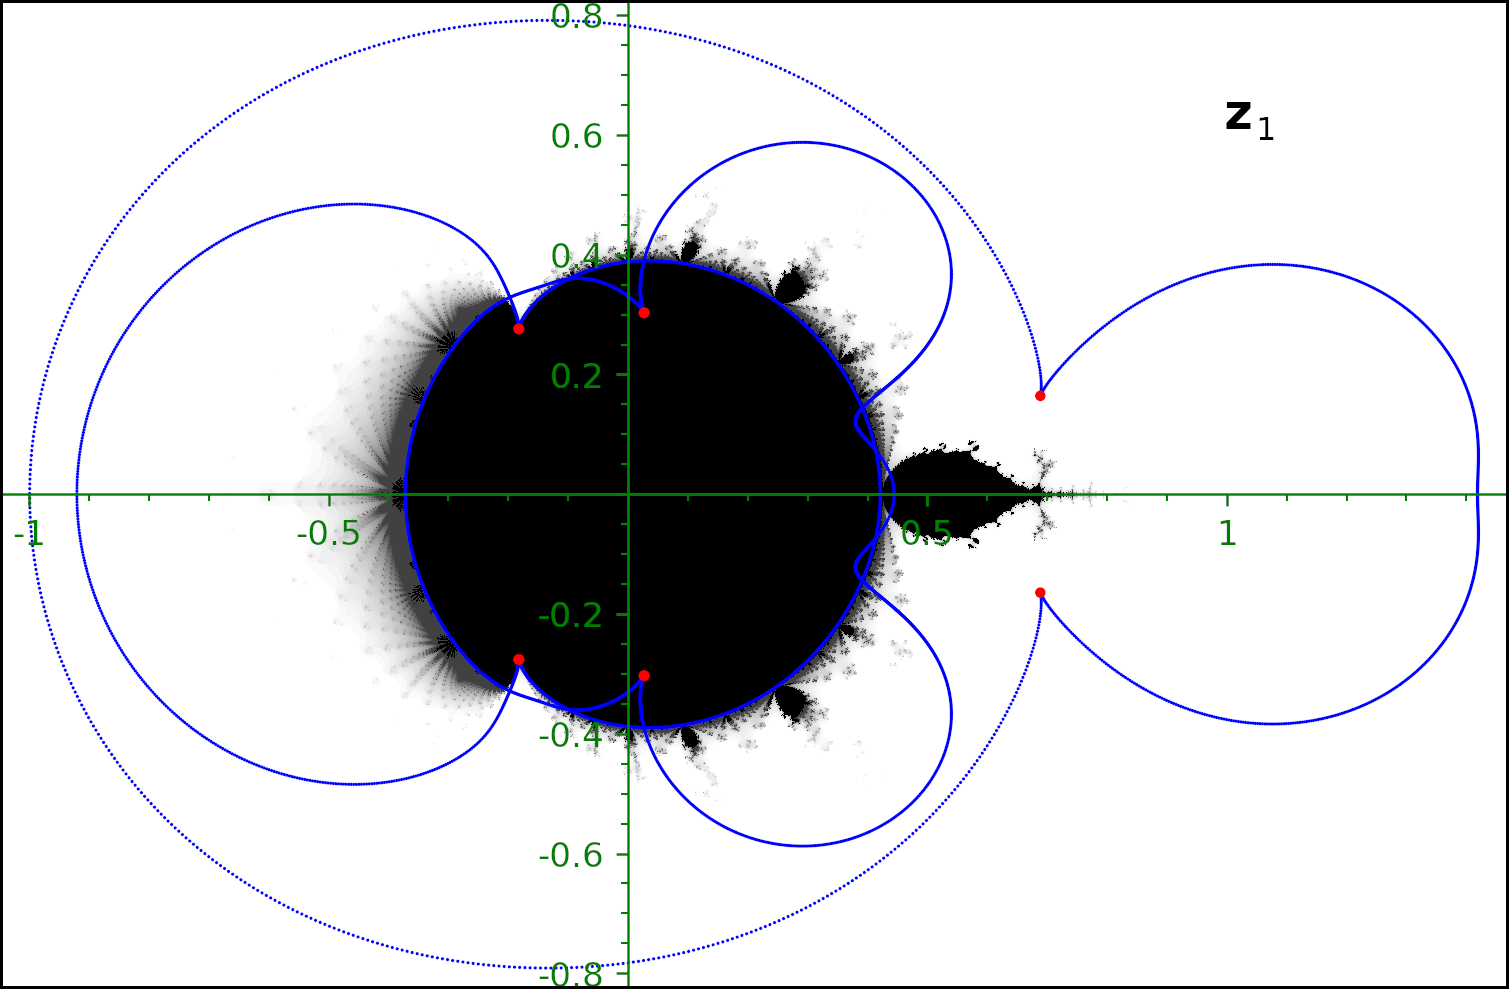
\includegraphics[width=0.70\columnwidth]{plots/figSIn1}
\caption{{The convergence domain on the~\(\lambda\)-plane for the first
column of~\(A\)~(the first eigenvector \(\mathbf z_1\))
for the~\(3\times3\) example. The Mandelbrot-like set (domain where orbits remain bounded) of the iterative scheme is shown in black and grey. The empirical convergence domain is shown in black. Its largest component corresponds to the stability of a steady state (the applicability domain of the iterative method). Small components correspond to stability of various periodic orbits. Various shades of grey show the values of $\lambda$ that lead to divergence to infinity (the darker the slower the divergence). In red are the values of $\lambda$ where the matrix is non-diagonalizable.
{\label{473965}}%%
}}
\end{center}
\end{figure}
\begin{figure}[H]
\begin{center}
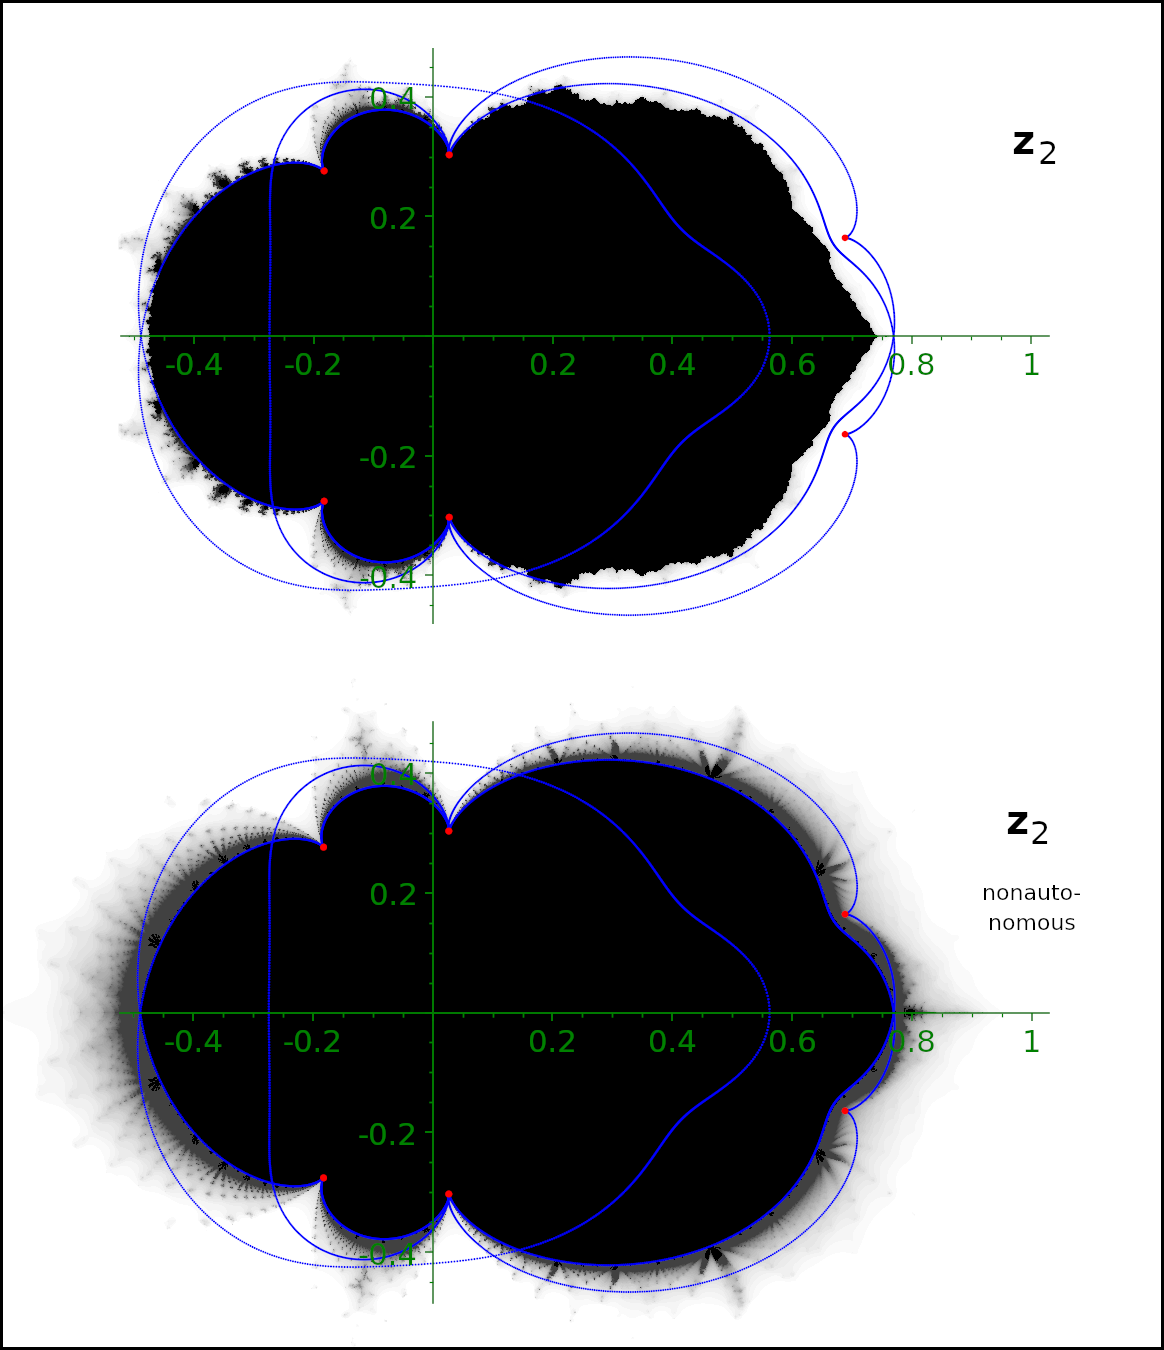
\includegraphics[width=0.70\columnwidth]{plots/figSIn2}
\caption{{{Same as ~{\cref{473965}} for the second
eigenvector~\(\mathbf z_2\) (the second column of \(A\)).
Small components correspond to stability of various periodic orbits.
Various shades of grey show the values of~\(\lambda\) that lead
to divergence to infinity (the darker the slower the divergence).
{\label{988969}}%
}%
}}
\end{center}
\end{figure}
\begin{figure}[H]
\begin{center}
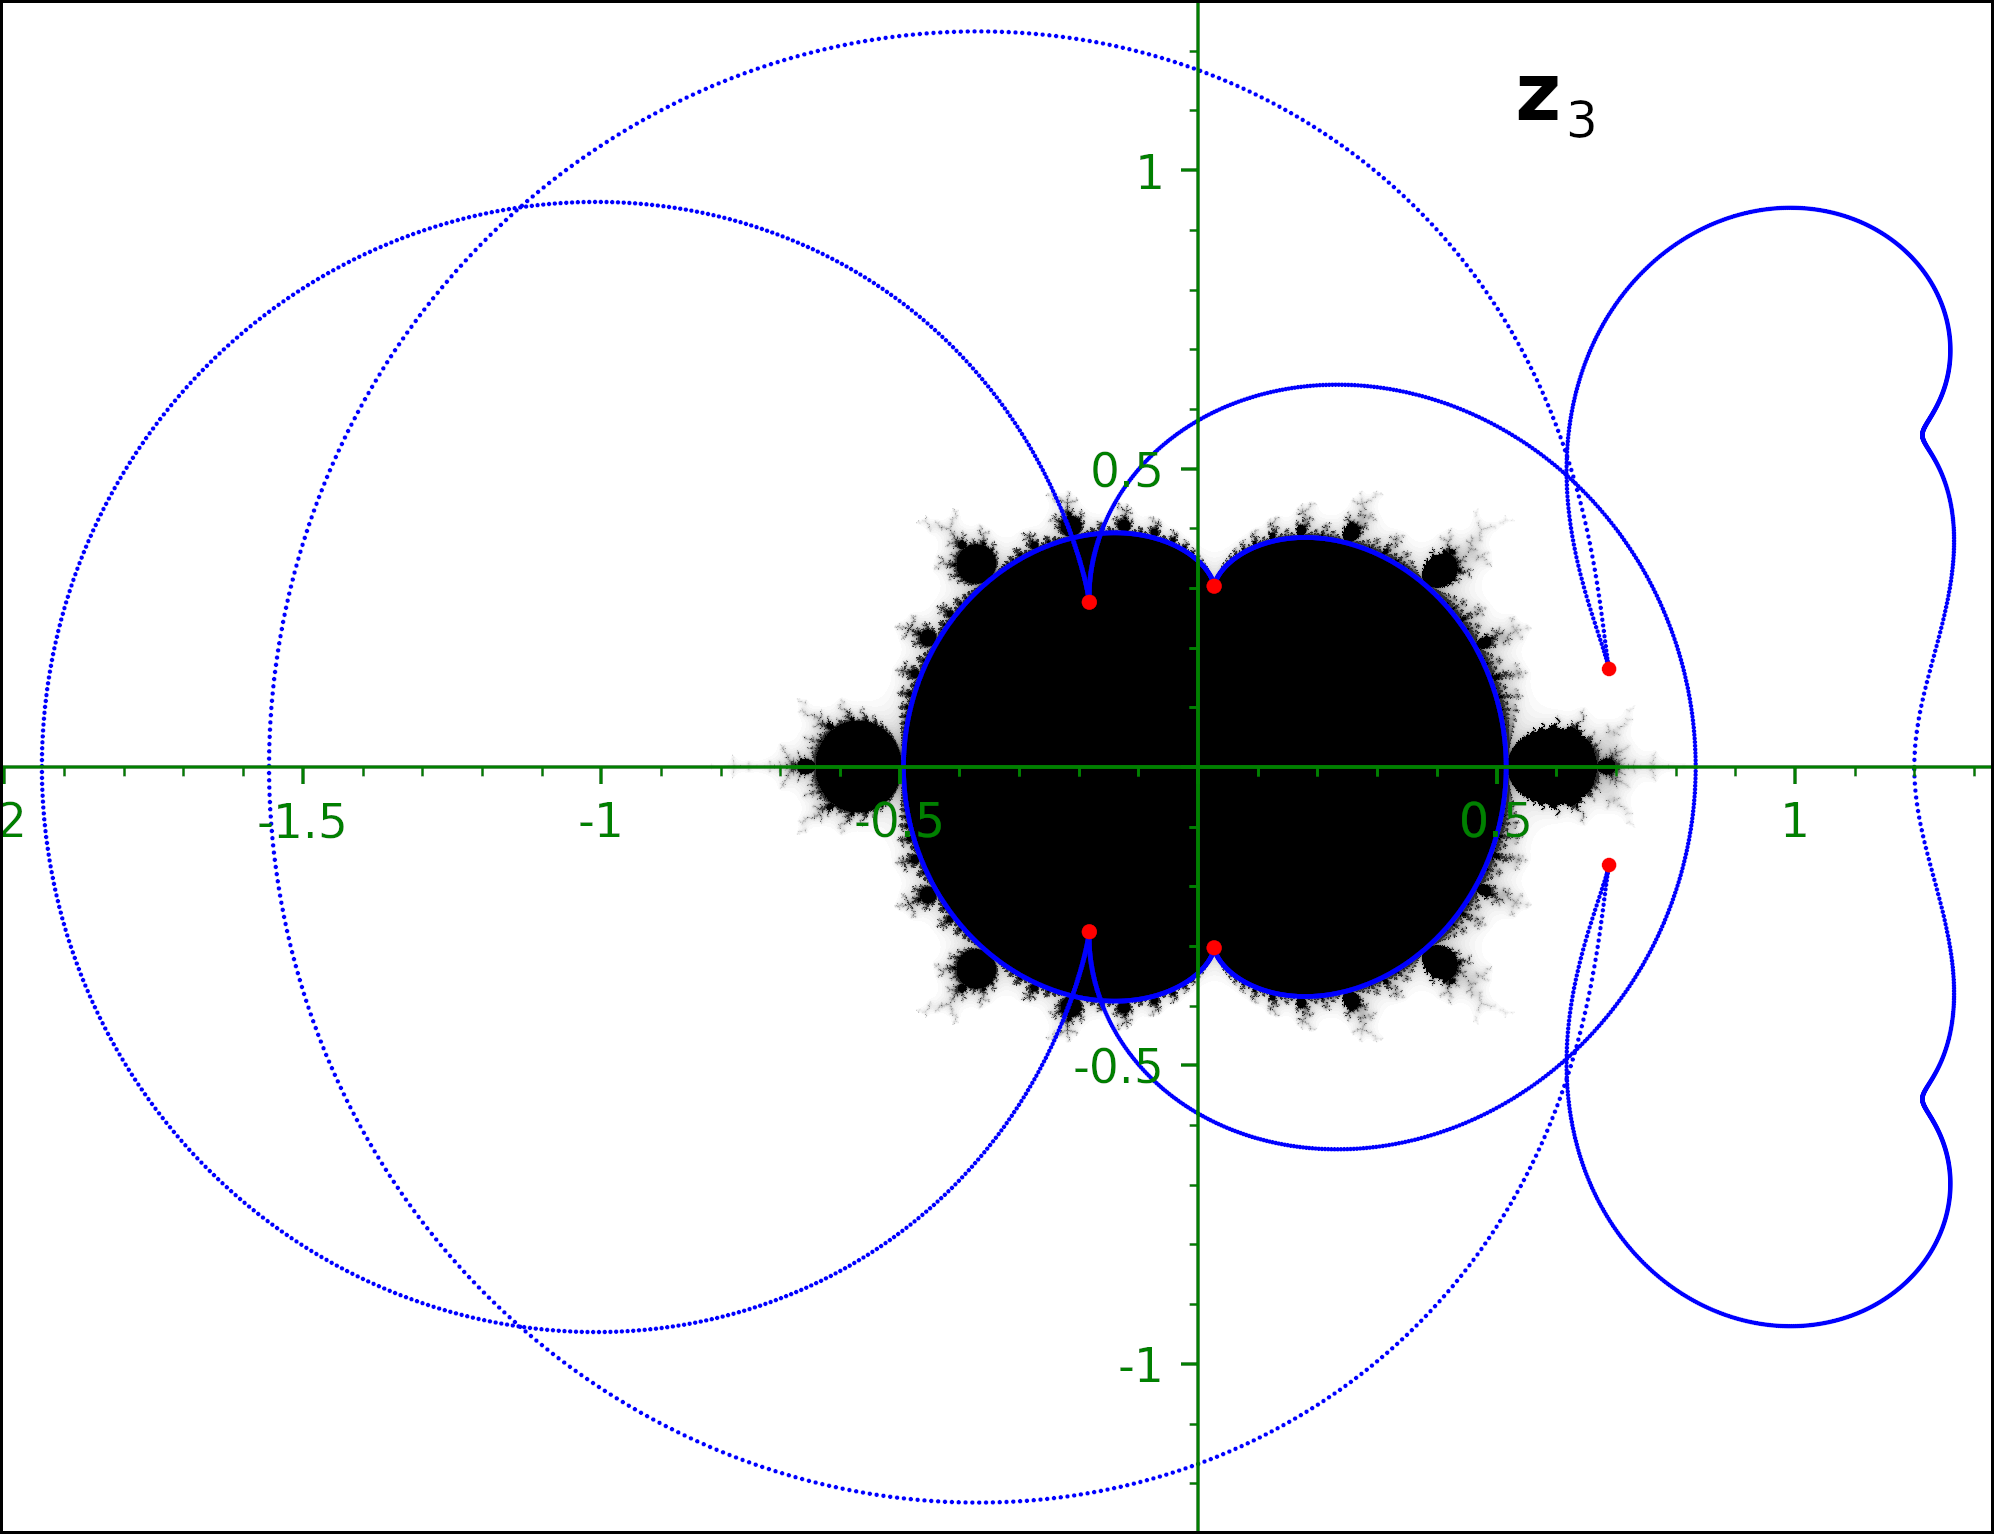
\includegraphics[width=0.70\columnwidth]{plots/figSIn3}
\caption{{{Same as ~{\cref{473965}} for the third
eigenvector~\(\mathbf z_3\) (the third column of~\(A\)) .
{\label{824432}}%
}%
}}
\end{center}
\end{figure}

\section{Exceptional points and cusps of $C$}\label{appendix:cusps}

In a large part of this section we drop the previously adopted notation conventions for vectors. We use instead the more appropriate notation style from differential geometry.

We will prove that if $M$ is defective at some value of $\lambda$, then $d\lambda/dt = 0$ for the curve $C$ at that point (as above, $\mu$ is a multiplier of the dynamical perturbation theory and $C$ is defined by $\mu = e^{it}$ and is locally considered as a curve $t \mapsto \lambda(t)$).

Fix $i$ and consider the dynamical system for the $i$-th column only. Let $\mathbf x = (x_1,\ldots,x_{n-1})$ be a tuple of affine coordinates in the affine chart $U_i$. Note that the coordinates are rearranged in comparison to $z_j$: $x_1 = z_1$, \ldots, $x_{i-1} = z_{i-1}$, $x_i = z_{i+1}$, \ldots, $x_{n-1} = z_n$. We consider the representation of the corresponding dynamical system in $U_i$ too. Let it be given by the tuple of functions $\mathbf h = (h_1,\ldots,h_{n-1})$ that correspond to functions in $\mathbf f_j$ with $(\mathbf f_i)_i$ omitted ($(\mathbf f_i)_i$ is trivially 1 in $U_i$). The same rearrangement is implied for $h_j$ as for $x_j$. Thus, the dynamical system is defined by $\mathbf x^{(k+1)} = \mathbf h(\mathbf x^{(k)})$ and the stationary states are defined by the system of equations $\mathbf x = \mathbf h(\mathbf x)$.

Consider $\mathbb C^{n+1}$ with coordinates $(x_1,\ldots,x_{n-1},\lambda,\nu)$, where $\nu \equiv \mu - 1$, as a complex analytic manifold with these coordinates as global holomorphic coordinates on it. Let us define polynomial functions
$$\mathcal F_j\colon \mathbb C^{n+1} \to \mathbb C, (\mathbf x,\lambda,\nu) \mapsto h_j(\mathbf x,\lambda) - x_j,$$
and $\mathbf {\mathcal F} = (\mathcal F_1,\ldots,\mathcal F_{n-1})$. Let us denote $J \equiv \dfrac{\D\mathcal F}{\D \mathbf x} \equiv \dfrac{\D(\mathcal F_1,\ldots,\mathcal F_{n-1})}{\D(x_1,\ldots,x_{n-1})}$ the Jacobian matrix of $\mathcal F$ with respect to variables $x_j$. Let $I$ be the unitary $(n-1)\times(n-1)$ matrix.

Consider the complex 1-dimensional variety $\mathcal C \subset \mathbb C^{n+1}$ defined by the polynomial system
$$
\begin{cases}
\mathcal F = 0,\\
\det(J - \nu I) = 0.
\end{cases}
$$
Curve $C$ is the projection to the $\lambda$-plane of the real 1-dimensional variety $\tilde C = \mathcal C \cap \{|\nu +1|^2 = 1\}$ in $\mathbb C^{N+1}$ considered as $\mathbb R^{2(N+1)}$.

First, note that if $M$ is defective at some value of $\lambda$, then the system of equations $\mathcal F = 0$ (with this values of $\lambda$ fixed and considered for unknowns $x \in \mathbb C^{n-1}$) has a root $x$ of multiplicity greater than 1. This means that the hyperplanes $\{\mathcal F_j =0\}$ are not in general position at the intersection that corresponds to this root, which implies $\det \D\mathcal F/\D \mathbf x = 0$. Therefore, the point $p \in \mathbb C^{n+1}$ with the same $x$ and $\lambda$ and with $\nu = 0$ belongs to $\mathcal C$ and represents this non-diagonalizability of $M$.

Let $d$ denote the exterior derivative and $\wedge$ denote the exterior product on the complex of holomorphic exterior forms $\Omega^\bullet(\mathbb C^{n+1})$. Alternatively, one may treat it in purely axiomatic way as the K\"ahler differential on the algebra of holomorphic functions on $\mathbb C^{n+1}$ with the appropriate factorization in the end. Let $p \in \mathcal C$ be a point of geometric degeneration of $M$ with $\nu = 0$ as above.

\begin{theorem}
Assume that the following nondegeneration condition holds: $d_p \det J \wedge \bigwedge\limits_j d_p \mathcal F_j \neq 0$. Then $\mathcal C$ can be locally parametrized by $\nu$ around $p$ and, with this parametrization, $d\lambda/d\nu = 0$ at $p$.
\end{theorem}

\begin{proof}
Let $T_p \mathbb C^{n+1}$ be the holomorphic tangent space to $\mathbb C^{n+1}$ at $p$, that is the tangent space spanned by the holomorphic vector fields $\D_j \equiv \D/\D x_j$, $\D_\lambda \equiv \D/\D \lambda$, $\D_\nu \equiv \D/\D \nu$ at $p$. Let us denote $\iota_u \sigma_p$ the contraction of a holomorphic form $\sigma$ ($\sigma_p \in \bigwedge^\bullet_p \mathbb C^{n+1}$) with a tangent vector $u \in T_p \mathbb C^{n+1}$ at point $p$.

Let us denote $\omega_p \equiv d_p \det (J - \nu I) \wedge \bigwedge\limits_j d_p \mathcal F_j$ and $\varpi_p \equiv d_p \det J \wedge \bigwedge\limits_j d_p \mathcal F_j$. By the premise, $\varpi_p \neq 0$, which also implies $\omega_p \neq 0$. Indeed, the free term (with respect to $\nu$) of the polynomial $\det(J - \nu I)$ is equal to $\det J$, and thus

\begin{equation}
d_p \det(J - \nu I) = \D_\nu \det(J - \nu I)|_p\, d_p \nu + d_p \det J,
\label{eq-nu} 
\end{equation}
where the two terms are linearly independent because $\D_\nu \det J = 0$. Therefore, as non of $\mathcal F_j$ depends on $\nu$, $\omega_p$ differs from $\varpi_p$ by an addition of a linearly independent term.

Let $v \in T_p \mathbb C^{n+1}$ be a nonzero vector with coordinates $(v^i,v^\lambda,v^\nu)$ tangent to $\mathcal C$. It means that $v\det (J - \nu I) = v\mathcal F_j = 0$, where by $vf$ we denote the action of a vector $v$ on a function $f$. This, in turn, implies $\iota_v \omega_p = 0$.

As all $\mathcal F_j$ depend only on $x$ and $\lambda$, we have $d_p \lambda \wedge \bigwedge\limits_j d_p \mathcal F_j = \det J|_p\, d_p \lambda \wedge \bigwedge\limits_j d_p x_j = 0$, and thus $d_p \lambda \wedge \omega_p = 0$. Therefore, we have
$$
\iota_v (d_p \lambda \wedge \omega_p) = -d_p \lambda \wedge \iota_v \omega_p + v^\lambda \omega_p = v^\lambda \omega_p = 0.
$$
This implies $v^\lambda = 0$.

On the other hand, by \cref{eq-nu} we have
$$d_p \nu \wedge d_p \det(J - \nu I) = d_p \nu \wedge d_p \det J,$$
and thus $d_p \nu \wedge \omega_p = d_p \nu \wedge \varpi_p \neq 0$. But $d \nu \wedge \omega \in \Omega^{n+1}(\mathbb C^{n+1})$, and therefore, for any holomorphic tangent vector $u \in T_p \mathbb C^{n+1}$, $u \neq 0$ is equivalent to $\iota_u (d_p \nu \wedge \omega_p) \neq 0$. This results in
$$
\iota_v (d_p \nu \wedge \omega_p) = -d_p \nu \wedge \iota_v \omega_p + v^\nu \omega_p = v^\nu \omega_p \neq 0,
$$
and thus $v^\nu \neq 0$.

By the holomorphic implicit function theorem, $\mathcal C$ can be holomorphically parametrized by $\nu$ in a neighborhood of $p$. Together with $v^\lambda = 0$ it implies that we have $d\lambda/d\nu|_p = 0$ on $\mathcal C$.
\end{proof}

Now, consider a smooth real curve parametrized by a real parameter $t$ on the complex $\nu$-plane that without degeneracy passes through 0. This curve is lifted to $\mathcal C$ and the resulting smooth real curve is parametrized by $t$. From $d\lambda/d\nu = 0$ we conclude that $d\lambda/dt = 0$ at $p$ too. In our case we have the curve $\mu(t) = e^{it}$ or $\nu(t) = e^{it} - 1$, which passes through $\mu = 1$ at $t = 0$. $\tilde C$ is projected without degeneration to $\mathbb C \times \mathbb R \ni (\lambda,t)$ locally near $p$ and then to $\mathbb C \ni \lambda$ with degeneration at the projection of $p$ given by $d\lambda/dt = 0$.



\end{document}